\documentclass[a4paper,12pt,twoside,final]{book}

\usepackage[utf8]{inputenc}

\usepackage[spanish,es-nodecimaldot]{babel} % International, rec. by RAE: http://www.tex-tipografia.com/marca_decimal.html

% Usar en TexStudio
%\usepackage[backend=bibtex, maxbibnames=99, giveninits=true]{biblatex}

% Usar en Overleaf
\usepackage[backend=biber, maxbibnames=99, giveninits=true]{biblatex}

\addbibresource{references.bib}
% COLOR
%\usepackage[usenames,dvipsnames,svgnames,table]{xcolor}
\usepackage{xcolor}



% Colores para estilo Proyecto Docente (tonos naranjas)
\definecolor{lightback}{HTML}{F4E0BF}
     \definecolor{back}{HTML}{F3C591}
\definecolor{lightline}{HTML}{FCAF5F}
     \definecolor{line}{HTML}{ED7900}
% Colores para portada
\definecolor{epsc:oscuro}{HTML}{280091}
 \definecolor{epsc:medio}{HTML}{4C5CC5}
 \definecolor{epsc:claro}{HTML}{3FCFD5}
 \definecolor{epsc:verde}{HTML}{00B299}




\usepackage{tikz} % used in cover to place images

\usepackage{datetime} % allow formal date format
% "Month, YEAR" date format, in spanish with the month uppercased not interfering other dates
\newcommand\Monthname[1][EMPTY]{
  \ifnum1=#1Enero\else
  \ifnum2=#1Febrero\else
  \ifnum3=#1Marzo\else
  \ifnum4=#1Abril\else
  \ifnum5=#1Mayo\else
  \ifnum6=#1Junio\else
  \ifnum7=#1Julio\else
  \ifnum8=#1Agosto\else
  \ifnum9=#1Septiembre\else
  \ifnum10=#1Octubre\else
  \ifnum11=#1Noviembre\else
  \ifnum12=#1Diciembre\else
  \fi\fi\fi\fi\fi\fi\fi\fi\fi\fi\fi\fi
}
\newdateformat{monthyeardate}{%
  \Monthname[\THEMONTH], \THEYEAR}


% FONTs
\usepackage[T1]{fontenc}
\usepackage{textcomp}           % Needed for new symbols like € ?

\usepackage[scaled]{berasans} % Font for the cover similar to Vera 33
%\renewcommand*\familydefault{\sfdefault}  %% To use as the base font of the document is to be sans serif


% PAGE STYLE
\usepackage[twoside,bindingoffset=0cm,headheight=30pt,margin=25mm]{geometry} %,verbose,showframe
\usepackage{fancyhdr} % Encabezados
\pagestyle{fancy}
\fancyhf{}
\fancyhead[LE]{\leftmark}
\fancyhead[RO]{\rightmark}
\fancyfoot[RO,LE]{\thepage}
% XXX Evitar el binding en la portada pero no en el resto del documento

% Sangría para párrafo, tabulaciones de 1 cm
\parindent=1.0cm
% Espacio o separación entre párrafos
\parskip 1.5ex

% TABLES AND FIGURES
\usepackage{graphicx}
\graphicspath{ {img/} }

\usepackage{todonotes}
\usepackage{float}
\usepackage{needspace}
\usepackage{tabularx}
\usepackage{url}
\usepackage{emptypage}
\usepackage[toc,page]{appendix}
\usepackage{hyperref}
\hypersetup{ colorlinks=true,                     %habilitar colorear enlaces
            linkcolor=black,
            filecolor=black,
            urlcolor=cyan,
            citecolor=blue,
            pdfborder={0 0 0},                    %sin borde en los enlaces
            breaklinks=true,                      %permitir saltos de línea en URLs
            }
\usepackage{array}
\usepackage{wrapfig}
\usepackage{multirow}
\usepackage{multicol} %Para poner columnas de un solo elemento
\usepackage{tabu}

\usepackage{pifont} %Para usar el vmark (tick) y xmark (cross)
\newcommand{\vmark}{\textcolor{green}{\ding{51}}} %Definición del vmark en verde
\newcommand{\xmark}{\textcolor{red}{\ding{55}}} %Definición del xmark en rojo

\usepackage{chngcntr}
\usepackage{verbatim}
\usepackage{graphicx}
\usepackage[export]{adjustbox}
\usepackage{listings}
\usepackage{minted}
\usepackage[final]{pdfpages}

\usepackage{booktabs,caption}
\usepackage[flushleft]{threeparttable}
\usepackage{fancyvrb}
\usepackage{verbatimbox}
\usepackage{afterpage}

\usepackage{csquotes}

\newsavebox{\FVerbBox}
\newenvironment{FVerbatim}
 {\VerbatimEnvironment
  \begin{center}
  \begin{lrbox}{\FVerbBox}
  \begin{BVerbatim}}
 {\end{BVerbatim}
  \end{lrbox}
  \fbox{\usebox{\FVerbBox}}
  \end{center}}
  
  
  \newcommand\blankpage{%
    \null
    \thispagestyle{empty}%
    \addtocounter{page}{-1}%
    \newpage}
    
\counterwithout{footnote}{chapter}
  
\begin{document}
\frontmatter

%------------- Cover --------------
\thispagestyle{empty}

% Backgroud images
\begin{tikzpicture}[remember picture, overlay]
  % Top
  \node [anchor=north east, inner sep=0pt]  at (current page.north east)
     {
\includegraphics[height=6cm]{imagen_uco/bottomLeftCorner.pdf}};
  % Bottom
  \node [anchor=south west, inner sep=0pt]  at (current page.south west)
     {
\includegraphics[height=6cm]{imagen_uco/bottomLeftCorner.pdf}};
  \node (uco) [anchor=south east, inner sep=0pt, xshift=-10mm, yshift=10mm]  at (current page.south east)
        {
\includegraphics[height=2cm]{imagen_uco/uco_debajo.pdf}};
  \node [anchor=south east, inner sep=0pt, xshift=-10mm]  at (uco.south west)
% Uncomment the chosen logo and comment the others:
        {
\includegraphics[height=2cm]{imagen_uco/bottomLeftCorner.pdf}};
%        {
\includegraphics[height=2cm]{imagen_uco/emblema-ing-industrial.pdf}};
%        {
\includegraphics[height=2cm]{imagen_uco/emblema-ing-tec-industrial.pdf}};
\end{tikzpicture}

\renewcommand*\listtablename{Índice de tablas}
\renewcommand{\tablename}{Tabla}
\begin{center}
\fontfamily{\sfdefault}\selectfont
\vspace*{2cm}

\vfill
\vfill

\includegraphics[width=12.5cm]{imagen_uco/LogotipoEPSC.pdf}
\vfill
\vfill

\large\textbf{\color{epsc:medio}
  TRABAJO FIN DE GRADO
}
\vfill
\Large\textbf{\color{epsc:verde}
  Especialidad de Computación
}
\vfill

\Large\textbf{\color{epsc:verde}
  Grado en Ingeniería Informática
}
\vfill
\vfill

\Huge\textbf{\color{epsc:oscuro}
       SimAS 3.0 descendente predictivo. Simulador de analizadores sintácticos descendentes predictivos.
}
\vfill
\vfill
\Large\textbf{\color{epsc:verde}
  Manual de usuario
}
\vfill
\vfill


\large{\color{epsc:oscuro}Autor}\\
\textbf{\color{epsc:medio}{D. Antonio Llamas García }}
\vfill

\large{\color{epsc:oscuro} Director }\\
\textbf{\color{epsc:medio} Prof. Dr. Nicolás Luis Fernández García }
\vfill



\textbf{\color{epsc:verde} \monthyeardate\today}
\vfill
\vfill
\vspace{2.7cm}
\end{center}


%-------------------------------------------------------------------------------------------------------
\clearpage

\thispagestyle{empty}
\pagecolor{white}

\cleardoublepage
%-------------------------------------------------------------------------------------------------------

\cleardoublepage
\setcounter{page}{1}
\setcounter{tocdepth}{3} %Numeración anidada de profundidad 3 en el índice
\setcounter{secnumdepth}{3} %Numeración anidada de profundidad 3 en los capítulos
\tableofcontents
\listoffigures
%\listoftables
%\cleardoublepage

\afterpage{\null\newpage}
\thispagestyle{empty}
\newpage
\mainmatter
%Insertar capitulos

%\part{Introducción e instalación del sistema}
\graphicspath{ {./img/capturas} }
\chapter{Introducción}

\section{Presentación}

La elección del lenguaje de programación adecuado es una decisión fundamental en el desarrollo de software. Este proceso implica considerar varios factores, como los requisitos del proyecto, la eficiencia, la facilidad de mantenimiento y la disponibilidad de herramientas y bibliotecas. Una vez seleccionado el lenguaje, surge la necesidad de traducir el código escrito en ese lenguaje a instrucciones que una computadora pueda entender y ejecutar.

La traducción del código se realiza a través de dos enfoques principales: compilación e interpretación. Estos enfoques difieren en su forma de transformar el código fuente en código ejecutable.

\subsection{Compilación}

La compilación implica la traducción del código de alto nivel a código máquina, que es el lenguaje específico de la computadora. Para ilustrar este proceso, consideremos un ejemplo simple en el lenguaje C:

\begin{verbatim}
#include <stdio.h>

int main() {
    printf("Hola, mundo!\n");
    return 0;
}
\end{verbatim}

Cuando compilamos este programa, el compilador traduce el código C a instrucciones específicas del procesador en código máquina. Estas instrucciones se almacenan en un archivo ejecutable, que puede ser ejecutado por la computadora.

\subsection{Interpretación}

En contraste, la interpretación implica ejecutar el código fuente directamente, línea por línea, sin generar un archivo ejecutable independiente. Un ejemplo común de un lenguaje interpretado es Python:

\begin{verbatim}
print("Hola, mundo!")
\end{verbatim}

En este caso, el intérprete de Python ejecuta cada línea de código a medida que se encuentra, generando la salida esperada sin producir un archivo ejecutable.

\subsection{Fases de traducción}

Tanto en la compilación como en la interpretación, el proceso de traducción consta de varias fases:

\begin{enumerate}
    \item \textbf{Análisis}: en esta fase se comprueba que el programa fuente está bien escrito.
    \begin{itemize}
        \item Análisis léxico: divide el código en componentes léxicos (\textit{tokens}) significativos.
        \item Análisis sintáctico: verifica la estructura gramatical del código.
        \item Análisis semántico: examina el significado y la coherencia del código.
    \end{itemize}
    
    \item \textbf{Síntesis}: esta fase se encarga de generar el código del programa ejecutable.
    \begin{itemize}
        \item Generación de código intermedio: crea una representación intermedia del código. Es una fase opcional pero recomendable.
        \item Optimización del código intermedio: permite mejora el código sin tener en cuenta el dispositivo donde se ejecutará. Es una fase opcional pero recomendable.
        \item Generación de código final: produce el código ejecutable o la salida del programa.
        \item Optimización: mejora el código para aumentar su eficiencia.
    \end{itemize}
\end{enumerate}

Estas fases aseguran que el código se traduzca de manera precisa y eficiente, garantizando su funcionamiento correcto.

Además, en el proceso de traducción, juegan un papel fundamental dos componentes auxiliares:

\begin{itemize}
    \item \textbf{Administrador de la tabla de símbolos}: este componente almacena información crucial sobre variables, funciones y otros elementos del programa. Proporciona un registro detallado que permite al traductor acceder y gestionar eficientemente los elementos del código fuente.
    
    \item \textbf{Gestor de errores}: este componente es esencial para manejar cualquier inconveniente que pueda surgir durante la traducción. Detecta y gestiona errores de sintaxis, semántica u otros problemas que podrían comprometer la integridad y funcionalidad del programa final.
\end{itemize}

En la Figura \ref{fig:fases}, se presenta un diagrama que resume las fases principales en el proceso de traducción, desde el análisis hasta la generación del código final.

\begin{figure}[htp]
    \centering
        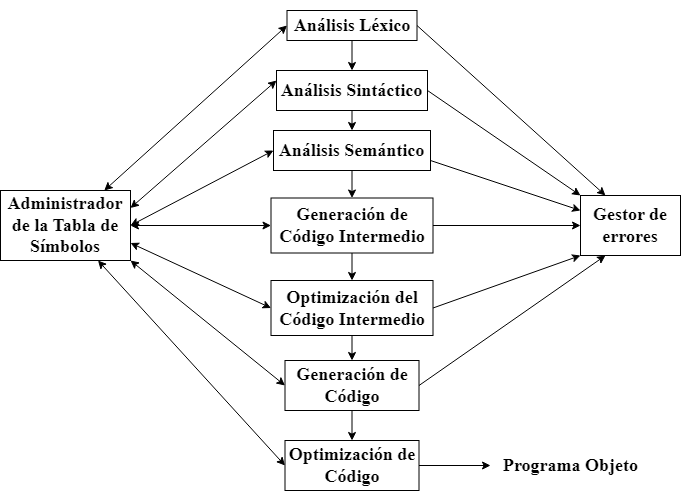
\includegraphics[scale=0.6]{figuras/Cap1/fasescomp.png} \\
    \caption{Fases Principales en el Proceso de Traducción}\label{fig:fases}
\end{figure}

\section{Definición del problema real}

Este proyecto de fin de carrera se enfoca en una tarea crucial: la corrección, mejora y ampliación de ``SimAS: Simuladores de Analizadores Sintácticos'', que es una aplicación desarrollada en java que tiene como objetivo ayudar a la docencia de la asignatura de Procesadores de Lenguajes de tercer curso de la especialidad de Computación del Grado de Ingeniería Informática. 

SimAS proporciona a los estudiantes una comprensión profunda del funcionamiento de la fase de análisis sintáctico en compiladores e intérpretes. Tiene la capacidad de simular tanto analizadores sintácticos descendentes como ascendentes, facilitando que los estudiantes comprendan mejor el funcionamiento de estos métodos de análisis sintáctico.

SimAS es una aplicación de software que posee dos versiones. SimAS 1.0 fue desarrollado por Vanesa González Pérez \cite{vanesa} como Proyecto de Fin de Carrera de Ingeniería Informática en 2015. Esta versión permitía realizar el análisis sintáctico descendente predictivo y el análisis ascendente LR (SLR, LR - canónico y LALR).  Esta versión fue corregida y ampliada en la versión SimAS 2.0, que fue desarrollada por Juan Antonio Fernández Díaz \cite{juan} en su Trabajo de Fin de Grado en 2023. Esta versión permitía generar informes en formato pdf y generar los árboles sintácticos asociados a la derivaciones de los analizadores sintácticos.


A pesar de la funcionalidad satisfactoria de SimAS, se han detectado una serie de errores y deficiencias que demandan atención inmediata.
\begin{itemize}
    \item Al cargar o modificar gramáticas, la aplicación debe ordenar sus reglas de producción en función del símbolo no terminal de la parte izquierda.
    \item Al crear o modificar gramáticas, la aplicación no genera bien el archivo XML \cite{xml} con dicha gramática.
    \item La aplicación no genera o genera de forma incorrecta los informes en formato PDF.
    \item No genera correctamente los conjuntos Primero y Siguiente de algunas gramáticas. Estos conjuntos son necesarios para realizar el análisis sintáctico descendente predictivo y el análisis sintáctico ascendente SLR.
    \item La aplicación no genera correctamente los árboles sintácticos asociados a las derivaciones.
    \item La interfaz produce algunas ventanas no interactivas o que no aportan valor.
\end{itemize}

Además, se pueden incorporar las siguientes mejoras para enriquecer la aplicación:

\begin{itemize}
    \item Diseñar una interfaz más intuitiva que genere todas las ventanas dentro de una misma interfaz y no en diferentes ventanas.
    \item Permitir el trabajo con varias gramáticas a la vez. 
    \item Implementar la posibilidad de cambiar el idioma de la aplicación.
\end{itemize}

Una descripción más detallada de las versiones de SimAS se puede consultar en el capítulo \ref{cap:antecedentes} de Antecedentes.


Aunque las versiones anteriores SimAS 1.0  y 2.0 permiten simular los análisis sintácticos descendente y ascendente, el presente Trabajo de Fin de Grado se va a centrar exclusivamente en corregir todos los fallos encontrados y en mejorar el análisis sintáctico descendente predictivo. La nueva aplicación se denominará ``SimAS 3.0 descendente predictivo''. Se considera que abordar también la corrección de los errores de la simulación del análisis sintáctico ascendente requeriría un esfuerzo superior al exigido en un Trabajo de Fin de Grado. Se debe tener en cuenta que la versión SimAS 2.0 \cite{juan} fue realizada en un Trabajo de Fin de Grado de doble especialidad que tiene una carga docente de 450 horas, superior a las 300 horas de un Trabajo de Fin de Grado de una única especialidad.


\section{Definición del problema técnico}


El presente Trabajo de Fin de Grado pretende desarrollar una aplicación informática multiplataforma, denominada ``SimAS 3.0 descendente predictivo'', que permita corregir y ampliar la simulación del análisis sintáctico descendente predictivo desarrollado en las versiones anteriores de SimAS 1.0 \cite{vanesa} y 2.0 \cite{juan}.

\subsection{Funcionamiento}
La aplicación propuesta se diseñará como una herramienta de escritorio multiplataforma con el objetivo de proporcionar a los usuarios una experiencia interactiva y educativa. Los principales módulos que integrará esta aplicación son los siguientes:

\begin{itemize}
    \item \textbf{Editor de gramáticas de contexto libre:} este módulo permitirá a los usuarios crear, cargar, guardar y modificar gramáticas de contexto libre. La interfaz proporcionará opciones intuitivas para trabajar con las reglas de producción, símbolos terminales y no terminales, así como la definición del símbolo inicial.

    \item \textbf{Simulador gráfico descendente:} esta funcionalidad simulará el proceso de análisis sintáctico descendente predictivo, utilizando la gramática especificada en el editor. El simulador generará una derivación por la izquierda y mostrará el árbol sintáctico descendente resultante.

    \item \textbf{Generación de árboles sintácticos descendentes:} se implementará la funcionalidad para generar árboles sintácticos de forma precisa y visualmente comprensible. Esta característica permitirá a los usuarios visualizar de manera clara la estructura jerárquica de las derivaciones sintácticas.
    
    \item \textbf{Tutorial interactivo:} este módulo proporcionará una guía paso a paso sobre los fundamentos y el funcionamiento de los métodos de análisis sintáctico. Los usuarios podrán acceder a explicaciones detalladas y ejemplos prácticos para comprender mejor los conceptos.
    
    \item \textbf{Ayuda integrada:} se incluirá una sección de ayuda en la interfaz para brindar asistencia instantánea sobre el uso de la aplicación. Los usuarios podrán acceder a información detallada sobre cada componente de la interfaz y los distintos módulos que componen la aplicación.
\end{itemize}

El funcionamiento detallado de cada uno de estos módulos se abordará en el capítulo \ref{cap:especificacion_requisitos} de Especificación de requisitos para proporcionar una comprensión completa de la aplicación.


\subsection{Entorno}
%Posibles modificaciones conforme se desarrolle la aplicación

El entorno en el que se desarrolla y ejecuta una aplicación es fundamental para garantizar su funcionalidad, usabilidad y despliegue efectivo. En este apartado, se detallan los aspectos relacionados con la interfaz de usuario, el entorno de desarrollo y el entorno de ejecución de la aplicación ``SimAS 3.0 descendente predictivo'', proporcionando una visión general de los componentes y requisitos clave para su funcionamiento.


\subsubsection{Interfaz con el usuario}

La aplicación contará con una interfaz gráfica de usuario (GUI\footnote{\textit{Graphical User Interface}}) diseñada para optimizar la experiencia del usuario, especialmente para los estudiantes. Se busca que todo el programa se ejecute en una única ventana, posibilitando la aparición de distintas pestañas, con el fin de simplificar la navegación. 

La interfaz estará diseñada para ser simple y completa al mismo tiempo, permitiendo a los usuarios realizar todas las operaciones necesarias para trabajar con gramáticas. Entre las funcionalidades específicas que ofrecerá la interfaz, se incluyen la capacidad de crear nuevas gramáticas e importar y editar gramáticas creadas previamente. Además, se proporcionará soporte para interacciones complejas, como la entrada de texto y la selección de archivos.

\subsubsection{Entorno de desarrollo}
El desarrollo y mantenimiento del código de la aplicación se realizará utilizando diversas fuentes de información disponibles en Internet, así como técnicas de inteligencia artificial. El entorno de desarrollo integrado (IDE) principal utilizado será IntelliJ \cite{intellij}, que ofrece una amplia gama de características y herramientas para el desarrollo de aplicaciones Java. Además, se utilizarán herramientas adicionales, como sistemas de control de versiones (Git \cite{git}) para el control del código fuente, y se gestionará la documentación y los recursos del proyecto en un repositorio de GitHub \cite{github}.

\subsubsection{Entorno de ejecución}
La aplicación estará diseñada para ser ejecutada en un entorno multiplataforma y compatible con los principales sistemas operativos, incluyendo Windows, macOS y Linux. No se requerirán configuraciones específicas del sistema operativo o del entorno de ejecución para garantizar el funcionamiento correcto de la aplicación. Además, la aplicación se ejecutará en una máquina virtual de Java \cite{java}, lo que proporcionará una mayor portabilidad y compatibilidad con diferentes sistemas. Esto significa que los usuarios finales no necesitarán instalar ninguna dependencia externa ni cumplir con requisitos adicionales de instalación, lo que facilitará su despliegue y uso.


\subsection{Ciclo de mantenimiento} \label{subsec:actualizaciones}

La gestión de actualizaciones de software es un proceso crítico que garantiza la evolución continua y la mejora de la aplicación a lo largo del tiempo. En el caso de ``SimAS 3.0 descendente predictivo'', se implementará un ciclo de mantenimiento diseñado para abordar nuevas funcionalidades, correcciones de errores y adaptaciones a los cambios en los entornos de ejecución.

El ciclo de mantenimiento de ``SimAS 3.0 descendente predictivo'' se basará en un enfoque proactivo y modular, permitiendo la incorporación de mejoras de manera eficiente y sin interrupciones significativas en la experiencia del usuario. Aunque el autor principal del proyecto no asumirá la responsabilidad directa del mantenimiento futuro, se establecerán procedimientos claros para la gestión de actualizaciones, asegurando la continuidad y la calidad del software.

Este enfoque modular no solo facilitará el mantenimiento y la actualización del software, sino que también fomentará la colaboración y la contribución de la comunidad de usuarios y desarrolladores. De esta manera, SimAS 3.0 podrá adaptarse de manera ágil a las necesidades cambiantes de los usuarios y a las demandas del entorno tecnológico.


\subsection{Competencia}

El desarrollo de SimAS 3.0 se sitúa en un contexto de continua evolución y expansión en el ámbito de las herramientas educativas para el análisis sintáctico en la informática. Aunque no buscamos competir comercialmente, es importante comprender el panorama actual y las características distintivas de SimAS 3.0 en relación con otras soluciones disponibles.

A través de un análisis exhaustivo en el Capítulo \ref{cap:antecedentes}, se explorará el terreno de las herramientas educativas existentes para el análisis sintáctico. Se examinarán tanto las aplicaciones desarrolladas en proyectos académicos previos, como otras soluciones disponibles en el mercado. Este análisis permitirá identificar fortalezas, debilidades y oportunidades de mejora para SimAS 3.0.

Si bien se reconocen las contribuciones de otras herramientas educativas, SimAS 3.0 buscará destacarse por su enfoque innovador y sus funcionalidades distintivas. Entre estas funcionalidades, se encuentra la capacidad de generar árboles sintácticos tanto descendentes como ascendentes, ofreciendo una experiencia de aprendizaje única y completa para los estudiantes de informática.


%Posibles modificaciones durante el desarrollo
\subsection{Aspecto externo}

En esta sección, se abordarán aspectos clave relacionados con la experiencia del usuario y la documentación asociada a SimAS 3.0.

\begin{itemize}
    \item \textbf{Diseño de la interfaz de usuario}: la interfaz de usuario de SimAS 3.0 se diseñará cuidadosamente para garantizar una experiencia visual atractiva y una navegación intuitiva. Se prestará especial atención a la disposición de los elementos, la coherencia visual y la accesibilidad, con el objetivo de proporcionar un entorno de trabajo cómodo y eficiente para los usuarios.
    
    \item \textbf{Documentación detallada}:
    \begin{itemize}
        \item \textit{Manual técnico}: este documento proporcionará una descripción exhaustiva de los aspectos técnicos del desarrollo de SimAS 3.0. Se incluirán detalles sobre la arquitectura del software, las tecnologías utilizadas y las decisiones de diseño fundamentales.
        
        \item \textit{Manual de usuario}: el manual de usuario de SimAS 3.0 contendrá instrucciones claras y concisas sobre la instalación, configuración y uso de la aplicación. Se incluirán ejemplos prácticos y capturas de pantalla para guiar al usuario a través de las diferentes funcionalidades de la aplicación.
        
        \item \textit{Manual de código}: este documento estará dirigido a desarrolladores y proporcionará una visión detallada del código fuente de SimAS 3.0. Se describirá la estructura del proyecto, las convenciones de codificación y la documentación interna del código para facilitar su comprensión y mantenimiento.
    \end{itemize}
    
    \item \textbf{Distribución y almacenamiento}: SimAS 3.0 estará disponible para su descarga en línea a través de un repositorio público, lo que facilitará el acceso a la última versión del software y de la documentación asociada. Además, se explorarán opciones para distribuir la aplicación en medios físicos o mediante servicios de almacenamiento en la nube, asegurando así su disponibilidad y accesibilidad para los usuarios.
\end{itemize}


\subsection{Estandarización}

En esta sección, se describirán los principios de diseño y usabilidad que guiarán el desarrollo de SimAS 3.0, con el objetivo de garantizar una experiencia de usuario coherente y satisfactoria.

\begin{itemize}
    \item \textbf{Diseño centrado en el usuario}: SimAS 3.0 se diseñará pensando en las necesidades y expectativas del usuario final. Se realizarán investigaciones de usuarios y pruebas de usabilidad para asegurar que la interfaz de usuario sea intuitiva y fácil de usar.
    
    \item \textbf{Consistencia y coherencia}: la interfaz de usuario de SimAS 3.0 mantendrá una apariencia y comportamiento coherentes en todas sus funciones y elementos. Se seguirán estándares de diseño reconocidos y se aplicarán patrones de diseño comunes para garantizar una experiencia consistente para el usuario.
    
    \item \textbf{Sensibilidad y guía del usuario}: la interfaz de SimAS 3.0 guiará al usuario a través de la aplicación, proporcionando retroalimentación clara y orientación en cada paso del proceso. Se utilizarán mensajes informativos y visuales para informar al usuario sobre el estado y las acciones disponibles.
    
    \item \textbf{Interacción intuitiva}: se priorizará una interacción sencilla y fluida en SimAS 3.0. Los controles y las funciones de la aplicación se diseñarán de manera intuitiva, minimizando la necesidad de aprendizaje por parte del usuario y facilitando el uso de la aplicación desde el primer momento.
    
    \item \textbf{Claridad y legibilidad}: la interfaz gráfica de SimAS 3.0 se diseñará con un enfoque en la claridad y la legibilidad. Se utilizarán colores y tipografías adecuados para garantizar una fácil comprensión de la información presentada, evitando la sobrecarga visual y la confusión del usuario.
\end{itemize}


\subsection{Calidad y fiabilidad}

En esta sección, se abordarán los aspectos de calidad, fiabilidad y seguridad que son fundamentales en el desarrollo y uso de SimAS 3.0. Se buscará garantizar el correcto funcionamiento de la aplicación, así como proteger la integridad y privacidad de los usuarios.

\begin{itemize}
    \item \textbf{Calidad y fiabilidad}: SimAS 3.0 se desarrollará con un enfoque en la calidad del software y la fiabilidad de su funcionamiento. Se utilizarán herramientas actualizadas como IntelliJ IDEA y la Máquina Virtual de Java para respaldar la calidad del código y su ejecución. Además, la aplicación será sometida a exhaustivas pruebas para detectar y corregir errores antes de su lanzamiento.
    
    \item \textbf{Seguridad}: la seguridad de SimAS 3.0 será una prioridad, tanto en términos de protección contra acciones incorrectas por parte del usuario como en la seguridad del dispositivo de almacenamiento. Se implementarán mecanismos de seguridad en la aplicación para evitar cualquier manipulación maliciosa o acceso no autorizado a los datos del usuario. Se garantizará que el usuario no tenga acceso a ninguna funcionalidad aparte de aquellas proporcionadas explícitamente por la aplicación, asegurando así que no se realicen acciones no deseadas ni se acceda a datos sensibles. Asimismo, se garantizará que la distribución y uso de la aplicación cumplan con los principios de software libre, siguiendo la licencia GPL de GNU para proteger su distribución y uso adecuados.
\end{itemize}


\subsection{Validación y verificación}

El proceso de validación y verificación de SimAS 3.0 es esencial para garantizar su correcto funcionamiento y la detección temprana de posibles errores.

\begin{itemize}
    \item \textbf{Validación}: se centrará en asegurar que la aplicación cumple con los requisitos y expectativas del usuario final. Se llevarán a cabo pruebas funcionales para verificar que todas las funcionalidades operan según lo esperado, y se realizarán pruebas de aceptación para garantizar que la aplicación satisface las necesidades del usuario.
    
    \item \textbf{Verificación}: por otro lado, se centrará en asegurar que el código y la lógica de la aplicación son correctos y libres de errores. Se realizarán pruebas unitarias para verificar el correcto funcionamiento de cada componente individualmente, así como pruebas de integración para garantizar que los componentes interactúan correctamente entre sí.
\end{itemize}

El proceso estará dividido en varias etapas, cada una con su respectiva documentación detallada:

\begin{itemize}
    \item \textbf{Planificación de pruebas}: se definirán los objetivos y alcance de las pruebas, así como los recursos y herramientas necesarios para llevarlas a cabo.
    
    \item \textbf{Diseño de pruebas}: se elaborará un plan detallado de las pruebas a realizar, incluyendo los casos de prueba específicos y los criterios de aceptación.
    
    \item \textbf{Ejecución de pruebas}: se llevarán a cabo las pruebas según el plan establecido, registrando los resultados obtenidos y cualquier incidencia detectada.
    
    \item \textbf{Análisis de resultados}: se analizarán los resultados de las pruebas para identificar posibles áreas de mejora o corrección. Se documentarán los errores encontrados y se propondrán soluciones para su resolución.
\end{itemize}

El capítulo \ref{cap:pruebas} detallará cada una de estas etapas y proporcionará una visión completa del proceso de validación y verificación de SimAS 3.0.


\subsection{Programa de tareas}

El desarrollo del Trabajo de Fin de Grado estará compuesto por las siguientes actividades:
\begin{enumerate}
    \item \textbf{Exploración inicial} 
        \begin{itemize}
            \item Comprensión y prueba de SimAS 2.0 \cite{juan}.
            \item Definición del problema técnico.
            \item Establecimiento de los objetivos.
            \item Revisión de los antecedentes.
            \item Identificación de los recursos iniciales y estratégicos.
            \item Selección de las herramientas de software y hardware.
            \item Investigación del entorno Intellij \cite{intellij} y del lenguaje de programación Java \cite{java}.
        \end{itemize}
    \item \textbf{Análisis y diseño}
        \begin{itemize}
            \item Especificación de requisitos: funcionales, no funcionales, de información y de la interfaz.
            \item Elaboración de los casos de uso.
            \item Validación de los casos de uso.
            \item Elaboración de los diagramas de secuencia.
        \end{itemize}
    \item \textbf{Diseño}
        \begin{itemize}
            \item Diseño de la arquitectura del sistema.
            \item Diseño de paquetes y clases.
            \item Diseño de la interfaz
        \end{itemize}        
    \item \textbf{Implementación}
        \begin{itemize}
            \item Desarrollo del código.
            \item Implementación de pruebas unitarias.
            \item Validación del código desarrollado.
        \end{itemize} 
    \item \textbf{Documentación}
      \begin{itemize}
          \item Elaboración del manual técnico, manual de usuario y manual de código.
          \item La redacción del manual técnico se realizará durante todo el proceso de desarrollo del Trabajo de Fin de Grado.
      \end{itemize}
\end{enumerate}

\subsection{Pruebas}
Las pruebas y la validación son elementos esenciales en el desarrollo de cualquier aplicación. Estos procesos permiten asegurar que la aplicación cumpla con los estándares de calidad y funcionalidad esperados. En el caso de SimAS 3.0, se llevarán a cabo diversas actividades de evaluación y validación para garantizar su correcto funcionamiento y fiabilidad.

\subsubsection{Tipos de Pruebas}

Se llevarán a cabo varios tipos de pruebas para evaluar distintos aspectos de SimAS 3.0:

\begin{itemize}
    \item \textbf{Pruebas de Funcionalidad:} estas pruebas se centran en verificar que todas las funciones y características de SimAS 3.0 funcionen como se espera. Se realizarán pruebas exhaustivas para cada módulo y componente de la aplicación.
    
    \item \textbf{Pruebas de Interfaz de Usuario:} estas pruebas se enfocarán en la usabilidad y la experiencia del usuario. Se evaluará la interfaz gráfica para garantizar que sea intuitiva y fácil de usar.

    \item \textbf{Pruebas de Rendimiento:} se llevarán a cabo pruebas para evaluar el rendimiento y la velocidad de SimAS 3.0, especialmente en situaciones de carga y con grandes conjuntos de datos.

    \item \textbf{Pruebas de Compatibilidad:} se realizarán pruebas en diferentes sistemas operativos y entornos de ejecución para garantizar que SimAS 3.0 funcione correctamente en diversas configuraciones.
\end{itemize}

\subsubsection{Descripción de las Pruebas}

Cada prueba estará estructurada de la siguiente manera:

\begin{itemize}
    \item \textbf{Objetivo:} se definirá claramente el objetivo de la prueba, es decir, qué se espera evaluar o validar.
    
    \item \textbf{Problema:} se identificarán y documentarán los problemas o errores detectados durante la ejecución de la prueba, junto con información detallada sobre cómo reproducirlos.

    \item \textbf{Solución:} se propondrán soluciones y acciones correctivas para abordar los problemas identificados durante las pruebas, asegurando así la mejora continua de la aplicación.
\end{itemize}

El próximo capítulo \ref{cap:pruebas} detallará los procedimientos y resultados de las pruebas llevadas a cabo en ``SimAS 3.0 descendente predictivo'' como parte de este Trabajo de Fin de Grado.


\subsection{Seguridad}
La seguridad en la presente aplicación se centra principalmente en garantizar su correcto funcionamiento sin comprometer la integridad de los sistemas donde se ejecute. Dado que la aplicación no maneja ni almacena datos personales de los usuarios, el enfoque de seguridad se orienta hacia la prevención de posibles daños a los equipos o entornos de ejecución.

Se implementarán medidas para asegurar que durante la ejecución de la aplicación, los usuarios no puedan realizar acciones que puedan comprometer su funcionamiento o la estabilidad del sistema. Además, se prestará especial atención a la protección del dispositivo de almacenamiento donde se ejecute la aplicación, garantizando que no se produzcan daños o alteraciones no deseadas.

En línea con la versión anterior, la aplicación se distribuirá libremente, sin restricciones de uso, copia o distribución. Esto se fundamenta en su naturaleza académica y en su carácter no lucrativo. No se aplicarán medidas de protección contra la distribución libre de la aplicación, permitiendo su acceso y uso por parte de cualquier usuario interesado en aprender o utilizarla con fines educativos.

En cuanto a la licencia, la aplicación seguirá los principios de la Licencia Pública General de GNU (GPL), que garantiza la libertad de uso, modificación y redistribución del software. Esta licencia ayuda a prevenir acciones malintencionadas relacionadas con la copia o reproducción del software, asegurando que permanezca accesible para la comunidad académica y de desarrollo de software.
\chapter{Instalación y desinstalación del programa}

\section{Requisitos}




\section{Ficheros de instalación}


\subsection{Instalación}


\subsection{Desinstalación}

\section{Estructura del programa ejecutable}

\section{Instalación de Graphviz}


\section{Ejecución de SimAS}

\chapter{Características de la interfaz}

\section{Introducción a la interfaz}

SimAS 3.0 presenta una interfaz moderna e intuitiva desarrollada con JavaFX \cite{javafx} que facilita el aprendizaje y uso de la aplicación. La interfaz está diseñada para ser clara, accesible y funcional, permitiendo a los usuarios concentrarse en los conceptos de análisis sintáctico sin distracciones innecesarias.

La aplicación utiliza un sistema de pestañas que permite trabajar con múltiples gramáticas y simulaciones simultáneamente, mejorando significativamente la productividad del usuario.

\section{Pantalla de bienvenida}

Al iniciar SimAS 3.0, la primera pantalla que aparece es la pantalla de bienvenida, que incluye:

\begin{itemize}
    \item \textbf{Logo de la aplicación}: identificación visual clara de SimAS 3.0.
    \item \textbf{Información de versión}: muestra la versión actual de la aplicación.
    \item \textbf{Credenciales del desarrollador}: información sobre el autor y director del proyecto.
    \item \textbf{Indicador de progreso}: muestra el estado de carga de los componentes de la aplicación.
\end{itemize}

Esta pantalla permanece visible durante unos segundos mientras la aplicación inicializa todos sus componentes y recursos necesarios.

\section{Menú principal}

Una vez completada la carga, la aplicación muestra el menú principal, que constituye el centro de navegación de SimAS 3.0.

\subsection{Elementos del menú principal}

El menú principal, mostrado en la figura \ref{fig:menu_principal}, incluye los siguientes elementos:

\begin{itemize}
    \item \textbf{Título de la aplicación}: \string"SimAS 3.0\string" en la parte superior.
    \item \textbf{Subtítulo}: \string"Simulador de Análisis Sintáctico\string" que describe la funcionalidad.
    \item \textbf{Botones de navegación}: acceso a las principales funcionalidades.
    \item \textbf{Selector de idioma}: en la esquina superior derecha.
    \item \textbf{Información del desarrollador}: en la parte inferior.
\end{itemize}

\needspace{8cm}
\begin{figure}[H]
    \centering
    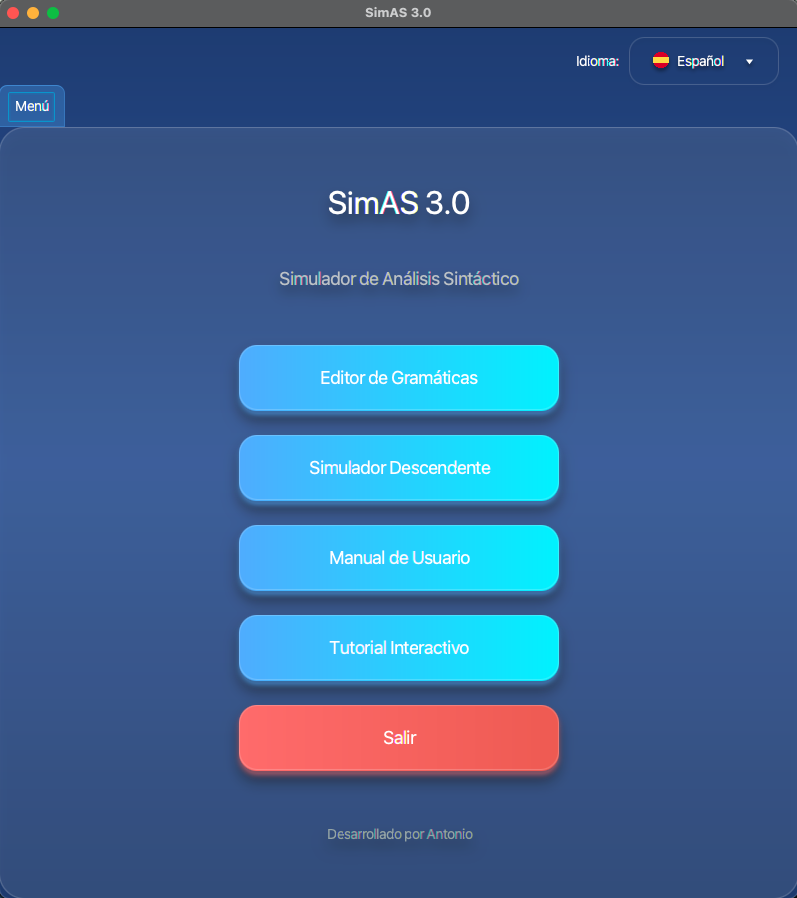
\includegraphics[width=0.9\textwidth]{figuras/menu.png}
    \caption{Menú principal de SimAS 3.0}
    \label{fig:menu_principal}
\end{figure}

\subsection{Botones principales}

Los botones del menú principal proporcionan acceso a las funcionalidades principales:

\begin{itemize}
    \item \textbf{Editor de gramáticas}: abre el editor para crear y gestionar gramáticas.
    \item \textbf{Simulador descendente}: accede al simulador de análisis sintáctico.
    \item \textbf{Manual de usuario}: abre este manual de usuario.
    \item \textbf{Tutorial interactivo}: proporciona una guía paso a paso.
    \item \textbf{Salir}: cierra la aplicación.
\end{itemize}

\section{Sistema de pestañas}

SimAS 3.0 implementa un sistema de pestañas avanzado que permite trabajar con múltiples elementos simultáneamente.

\subsection{Características del sistema de pestañas}

\begin{itemize}
    \item \textbf{Pestaña principal}: siempre visible, contiene el menú principal.
    \item \textbf{Pestañas dinámicas}: se crean automáticamente al abrir editores o simuladores.
    \item \textbf{Numeración automática}: las pestañas se numeran secuencialmente para facilitar la identificación.
    \item \textbf{Cierre individual}: cada pestaña puede cerrarse independientemente.
    \item \textbf{Reordenamiento}: las pestañas pueden arrastrarse para cambiar su orden.
\end{itemize}

\subsection{Gestión de pestañas}

\begin{itemize}
    \item \textbf{Botón \string"Cerrar todas las pestañas\string"}: cierra todas las pestañas excepto la principal.
    \item \textbf{Menú contextual}: clic derecho en una pestaña para opciones adicionales.
    \item \textbf{Separación de pestañas}: arrastrar una pestaña fuera del área principal crea una nueva ventana.
    \item \textbf{Reunión de ventanas}: arrastrar pestañas entre ventanas las consolida.
    \item \textbf{Grupos de pestañas}: las pestañas relacionadas (editor y simulador) se agrupan automáticamente.
    \item \textbf{Movimiento de grupos}: arrastrar una pestaña de un grupo mueve todo el grupo a una nueva ventana.
    \item \textbf{Numeración de grupos}: cada grupo de pestañas recibe un número único para identificación.
\end{itemize}

\section{Selector de idioma}

SimAS 3.0 soporta múltiples idiomas, permitiendo a los usuarios trabajar en su idioma preferido.

\subsection{Idiomas disponibles}

La aplicación incluye soporte para los siguientes idiomas:

\begin{itemize}
    \item \textbf{Español}: idioma por defecto.
    \item \textbf{English}: inglés.
    \item \textbf{Français}: francés.
    \item \textbf{Português}: portugués.
    \item \textbf{Deutsch}: alemán.
    \item \textbf{Japanese}: japonés.
\end{itemize}

\subsection{Cambio de idioma}

Para cambiar el idioma de la interfaz:

\begin{enumerate}
    \item Localice el selector de idioma en la esquina superior derecha de la ventana principal de la aplicación.
    \item Haga clic en el menú desplegable.
    \item Seleccione el idioma deseado de la lista.
    \item La interfaz se actualizará inmediatamente al nuevo idioma.
    \item El cambio se aplicará a todas las pestañas y ventanas abiertas.
    \item El idioma seleccionado se mantiene durante toda la sesión de trabajo.
\end{enumerate}

\needspace{8cm}
\begin{figure}[H]
    \centering
    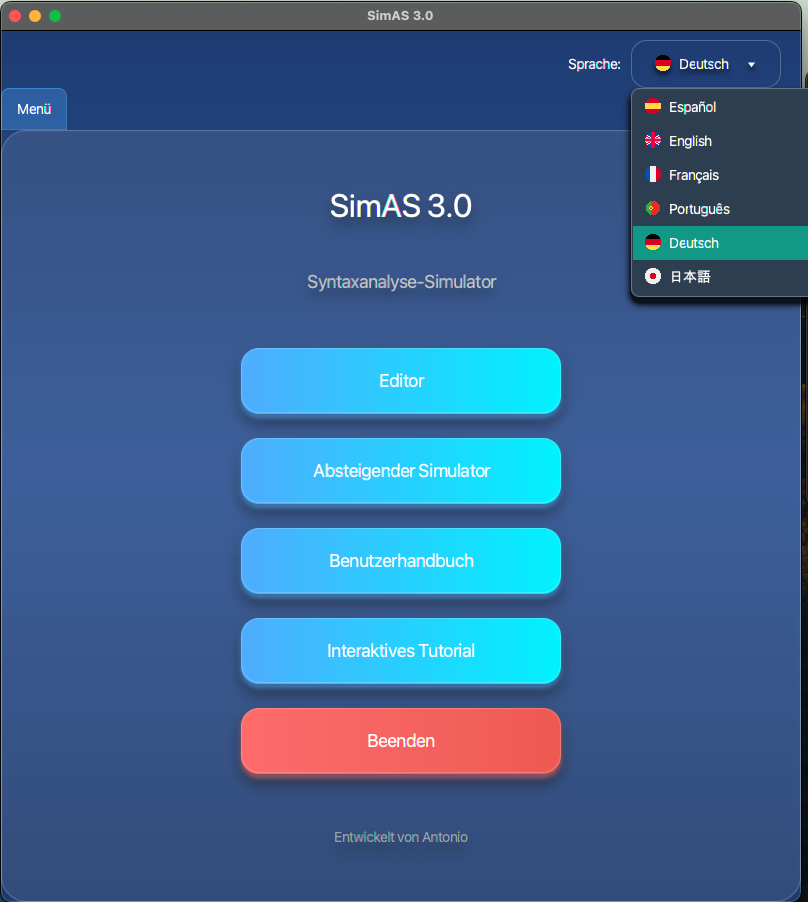
\includegraphics[width=0.9\textwidth]{figuras/menu_idiomas.png}
    \caption{Selector de idiomas con menú desplegable}
    \label{fig:menu_idiomas}
\end{figure}

El selector de idiomas, ilustrado en la figura \ref{fig:menu_idiomas}, muestra todos los idiomas disponibles en un menú desplegable fácil de usar.

\section{Atajos de teclado}

SimAS 3.0 incluye atajos de teclado para facilitar el acceso rápido a las funciones principales.

\subsection{Atajos disponibles}

SimAS 3.0 incluye los siguientes atajos de teclado:

\begin{itemize}
    \item \textbf{Ctrl+N}: abre el editor de gramáticas.
    \item \textbf{Ctrl+S}: abre el simulador descendente.
    \item \textbf{Ctrl+H}: abre el manual de usuario.
    \item \textbf{Ctrl+W}: cierra la pestaña actual.
    \item \textbf{Ctrl+Shift+W}: cierra todas las pestañas. 
    \item \textbf{Ctrl+Tab}: navega a la siguiente pestaña.
    \item \textbf{Ctrl+Shift+Tab}: navega a la pestaña anterior.
    \item \textbf{Ctrl+T}: crea una nueva pestaña del editor.
    \item \textbf{Ctrl+Shift+T}: crea una nueva ventana.
    \item \textbf{Ctrl+1-9}: navega directamente a la pestaña numerada.
\end{itemize}

\subsection{Uso de atajos}

Los atajos de teclado funcionan desde cualquier pestaña activa y proporcionan acceso rápido a las funcionalidades más utilizadas, mejorando la eficiencia del usuario.

\section{Elementos visuales}

La interfaz de SimAS 3.0 utiliza elementos visuales consistentes para mejorar la experiencia del usuario.

\subsection{Iconos y gráficos}

\begin{itemize}
    \item \textbf{Iconos descriptivos}: cada botón principal incluye un icono que representa su función.
    \item \textbf{Banderas de países}: el selector de idioma muestra banderas para identificación visual.
    \item \textbf{Indicadores de estado}: elementos visuales que muestran el estado de las operaciones.
    \item \textbf{Colores consistentes}: paleta de colores coherente en toda la aplicación.
\end{itemize}

\subsection{Tipografía y espaciado}

\begin{itemize}
    \item \textbf{Fuentes legibles}: tipografía clara y fácil de leer.
    \item \textbf{Espaciado apropiado}: elementos bien distribuidos para evitar saturación visual.
    \item \textbf{Jerarquía visual}: diferentes tamaños de fuente para establecer importancia.
    \item \textbf{Contraste adecuado}: colores que facilitan la lectura.
\end{itemize}

\section{Responsividad de la interfaz}

La interfaz de SimAS 3.0 está diseñada para adaptarse a diferentes tamaños de pantalla y resoluciones.

\subsection{Adaptación a la pantalla}

\begin{itemize}
    \item \textbf{Tamaño mínimo}: la ventana puede redimensionarse hasta 600x700 píxeles.
    \item \textbf{Tamaño por defecto}: 800x900 píxeles para una experiencia óptima.
    \item \textbf{Escalado automático}: los elementos se adaptan al tamaño de la ventana.
    \item \textbf{Barras de desplazamiento}: aparecen automáticamente cuando es necesario.
\end{itemize}

\subsection{Optimización para diferentes resoluciones}

La aplicación se optimiza automáticamente para:

\begin{itemize}
    \item \textbf{Resoluciones estándar}: 1024x768, 1366x768, 1920x1080.
    \item \textbf{Pantallas de alta densidad}: soporte para pantallas Retina y similares.
    \item \textbf{Orientaciones}: funciona correctamente en orientación horizontal.
    \item \textbf{Proporciones}: se adapta a diferentes relaciones de aspecto.
\end{itemize}

\section{Accesibilidad}

SimAS 3.0 incluye características de accesibilidad para facilitar su uso por parte de todos los usuarios.

\subsection{Características de accesibilidad}

\begin{itemize}
    \item \textbf{Atajos de teclado}: alternativa al uso del ratón.
    \item \textbf{Contraste visual}: colores que facilitan la distinción de elementos.
    \item \textbf{Tamaño de fuente}: texto legible en diferentes tamaños de pantalla.
    \item \textbf{Navegación por teclado}: todos los elementos son accesibles mediante teclado.
\end{itemize}

\subsection{Compatibilidad con tecnologías asistivas}

La aplicación es compatible con:

\begin{itemize}
    \item \textbf{Amplificadores de pantalla}: elementos visuales claros y contrastados.
    \item \textbf{Dispositivos de entrada alternativos}: soporte para diferentes tipos de entrada (ratón, teclado, trackpad).
    \item \textbf{Software de control por voz}: compatible con sistemas de control por voz del sistema operativo.
    \item \textbf{Dispositivos de entrada adaptativos}: soporte para dispositivos especializados de accesibilidad.
\end{itemize}

\section{Personalización de la interfaz}

Aunque SimAS 3.0 mantiene una apariencia consistente, los usuarios pueden personalizar algunos aspectos de la experiencia.

\subsection{Opciones de personalización}

\begin{itemize}
    \item \textbf{Idioma}: selección del idioma de la interfaz.
    \item \textbf{Tamaño de ventana}: redimensionamiento según preferencias.
    \item \textbf{Organización de pestañas}: reordenamiento y agrupación.
    \item \textbf{Atajos de teclado}: uso opcional de atajos para funciones rápidas.
\end{itemize}

\subsection{Limitaciones de personalización}

Por motivos de consistencia y funcionalidad, algunos elementos no son personalizables:

\begin{itemize}
    \item \textbf{Colores de la interfaz}: paleta fija para mantener coherencia visual.
    \item \textbf{Tipografía}: fuente estándar para garantizar legibilidad.
    \item \textbf{Disposición de elementos}: estructura fija para optimizar el flujo de trabajo.
    \item \textbf{Iconos}: conjunto estándar para facilitar el reconocimiento.
\end{itemize}

\section{Integración entre componentes}

La interfaz de SimAS 3.0 está diseñada para facilitar la integración entre diferentes componentes de la aplicación.

\subsection{Flujo de trabajo integrado}

\begin{itemize}
    \item \textbf{Editor a simulador}: transición directa desde el editor al simulador.
    \item \textbf{Sincronización de datos}: las gramáticas se comparten automáticamente entre componentes.
    \item \textbf{Estado consistente}: cambios en un componente se reflejan en otros.
    \item \textbf{Navegación fluida}: transiciones suaves entre diferentes funcionalidades.
\end{itemize}

\subsection{Comunicación entre ventanas}

\begin{itemize}
    \item \textbf{Ventanas secundarias}: creación de ventanas adicionales para trabajo paralelo.
    \item \textbf{Sincronización de idioma}: cambios de idioma se aplican a todas las ventanas.
    \item \textbf{Gestión de estado}: estado compartido entre ventanas relacionadas.
    \item \textbf{Cierre coordinado}: cierre apropiado de ventanas dependientes.
\end{itemize}

\section{Solución de problemas de interfaz}

Si experimenta problemas con la interfaz de SimAS 3.0, considere las siguientes soluciones:

\subsection{Problemas comunes}

\begin{itemize}
    \item \textbf{Interfaz no se muestra correctamente}: verifique la resolución de pantalla y actualice los controladores gráficos.
    \item \textbf{Elementos superpuestos}: redimensione la ventana o cambie la resolución de pantalla.
    \item \textbf{Texto borroso}: ajuste la configuración de escalado de Windows/macOS.
    \item \textbf{Atajos de teclado no funcionan}: asegúrese de que la ventana esté activa y enfocada.
\end{itemize}

\subsection{Optimización del rendimiento}

Para obtener el mejor rendimiento de la interfaz:

\begin{itemize}
    \item \textbf{Cierre pestañas innecesarias}: mantenga solo las pestañas que esté utilizando.
    \item \textbf{Resolución apropiada}: use una resolución de pantalla compatible.
    \item \textbf{Memoria disponible}: asegúrese de tener suficiente memoria RAM libre.
    \item \textbf{Controladores actualizados}: mantenga actualizados los controladores gráficos.
\end{itemize}

\section{Ventanas secundarias}

SimAS 3.0 permite crear ventanas secundarias para trabajar con múltiples proyectos simultáneamente, mejorando significativamente la productividad del usuario.

\subsection{Creación de ventanas secundarias}

Las ventanas secundarias se pueden crear de las siguientes maneras:

\begin{itemize}
    \item \textbf{Arrastrando pestañas}: arrastrar una pestaña fuera del área principal crea automáticamente una nueva ventana.
    \item \textbf{Menú contextual}: clic derecho en una pestaña y seleccionar \string"Nueva ventana\string".
\end{itemize}

\subsection{Características de las ventanas secundarias}

Cada ventana secundaria mantiene las siguientes características:

\begin{itemize}
    \item \textbf{Independencia}: cada ventana funciona de manera independiente.    
    \item \textbf{Sincronización de idioma}: cambios de idioma se aplican a todas las ventanas.
    \item \textbf{Gestión de pestañas}: cada ventana tiene su propio sistema de pestañas.
    \item \textbf{Estado persistente}: el estado de cada ventana se mantiene durante la sesión.
    \item \textbf{Comunicación entre ventanas}: las ventanas pueden compartir datos cuando es necesario.
\end{itemize}

\subsection{Gestión de múltiples ventanas}

Para gestionar eficientemente múltiples ventanas:

\begin{itemize}
    \item \textbf{Organización}: cada ventana puede contener un proyecto diferente.
    \item \textbf{Intercambio de datos}: arrastrar pestañas entre ventanas para reorganizar el trabajo.
    \item \textbf{Cierre coordinado}: cerrar una ventana principal cierra todas las ventanas secundarias.
\end{itemize}

\section{Barra de estado y notificaciones}

SimAS 3.0 incluye una barra de estado que proporciona información importante sobre el estado de la aplicación y las operaciones en curso.

\subsection{Elementos de la barra de estado}

La barra de estado incluye:

\begin{itemize}
    \item \textbf{Mensajes informativos}: notificaciones sobre el estado del sistema.
    \item \textbf{Contador de pestañas}: número total de pestañas abiertas.
    \item \textbf{Indicador de idioma}: idioma actualmente seleccionado.
\end{itemize}

\subsection{Sistema de notificaciones}

El sistema de notificaciones proporciona:

\begin{itemize}
    \item \textbf{Notificaciones de éxito}: confirmación de operaciones completadas.
    \item \textbf{Advertencias}: alertas sobre posibles problemas.
    \item \textbf{Errores}: información detallada sobre errores encontrados.
    \item \textbf{Información contextual}: ayuda específica según la situación.
\end{itemize}

\section{Menús contextuales}

SimAS 3.0 implementa menús contextuales inteligentes que se adaptan al contexto actual.

\subsection{Menús contextuales de pestañas}

Al hacer clic derecho en una pestaña, se muestra un menú con opciones como:

\begin{itemize}
    \item \textbf{Cerrar pestaña}: cierra la pestaña actual.
    \item \textbf{Cerrar todas las pestañas}: cierra todas las pestañas de la ventana actual.
    \item \textbf{Abrir en nueva ventana}: abre la pestaña en una nueva ventana.
    \item \textbf{Abrir en ventana existente}: abre la pestaña en una ventana existente.
\end{itemize}


\section{Conclusión}

La interfaz de SimAS 3.0 está diseñada para proporcionar una experiencia de usuario intuitiva, eficiente y profesional. Con su sistema de pestañas avanzado, soporte multiidioma completo, atajos de teclado extensivos, características de accesibilidad robustas e integración profunda con el sistema operativo, la aplicación facilita el aprendizaje y uso de los conceptos de análisis sintáctico descendente predictivo.

La capacidad de trabajar con múltiples elementos simultáneamente, la gestión inteligente de ventanas secundarias, los menús contextuales adaptativos y la configuración avanzada hacen de SimAS 3.0 una herramienta poderosa, flexible y profesional para estudiantes, profesores e investigadores en el campo de la informática y la teoría de lenguajes formales.

La interfaz no solo cumple con los estándares de usabilidad modernos, sino que también establece nuevas referencias en el campo de las aplicaciones educativas especializadas, proporcionando una experiencia de usuario a la altura de las mejores herramientas profesionales del mercado.
\input{capitulos/04_Editor_Gramática}
\chapter{Simulación del analizador descendente predictivo}

El simulador de análisis sintáctico descendente predictivo representa el núcleo tecnológico más sofisticado de SimAS 3.0, diseñado específicamente para simular y visualizar el proceso completo de análisis sintáctico de gramáticas libres de contexto utilizando el algoritmo LL(1). Este componente avanzado no solo ejecuta el análisis, sino que proporciona una experiencia educativa inmersiva que permite a los usuarios comprender profundamente los mecanismos internos del análisis sintáctico predictivo, desde la construcción de la tabla de análisis hasta la ejecución paso a paso del algoritmo.

\section{Introducción al simulador}

El simulador de SimAS 3.0 implementa un analizador descendente predictivo de última generación que utiliza una tabla de análisis precomputada para determinar de manera determinista qué producción aplicar en cada paso del análisis. Este enfoque algorítmico avanzado garantiza un análisis eficiente y completamente determinista de las cadenas de entrada, siempre que la gramática cumpla con las condiciones LL(1). La implementación incluye optimizaciones específicas para el manejo de gramáticas complejas y sistemas de recuperación de errores robustos que mejoran significativamente la experiencia del usuario.

\subsection{Características principales}

El simulador incorpora un conjunto integral de funcionalidades avanzadas que lo convierten en una herramienta educativa y profesional de primer nivel:

\begin{itemize}
    \item \textbf{Asistente guiado inteligente}: proceso de configuración estructurado en 5 pasos secuenciales con validación automática en tiempo real y retroalimentación inmediata sobre la corrección de cada transformación.
    \item \textbf{Refactorización automática avanzada}: eliminación sistemática de recursividad izquierda directa e indirecta, factorización de producciones con prefijos comunes, y optimización de la estructura gramatical para análisis LL(1).
    \item \textbf{Cálculo de conjuntos PRIMERO y SIGUIENTE}: generación automática y eficiente de los conjuntos fundamentales utilizando algoritmos optimizados que manejan gramáticas de cualquier complejidad.
    \item \textbf{Construcción de tabla predictiva}: generación automática de la tabla de análisis LL(1) con detección de conflictos y sugerencias de resolución.
    \item \textbf{Sistema de funciones de error}: implementación de un sistema avanzado de recuperación de errores con funciones predefinidas y capacidad de personalización completa.
    \item \textbf{Simulación interactiva completa}: análisis paso a paso con control granular del usuario, incluyendo avance, retroceso, pausa y reinicio en cualquier momento del proceso.
    \item \textbf{Visualización dinámica}: generación automática de derivaciones en formato BNF y árboles sintácticos que se actualizan en tiempo real durante la simulación.
    \item \textbf{Múltiples simulaciones concurrentes}: capacidad de ejecutar y gestionar múltiples simulaciones simultáneamente para análisis comparativo y validación exhaustiva.
\end{itemize}

\section{Acceso al simulador}

El simulador está diseñado con múltiples puntos de acceso estratégicos que facilitan su uso en diferentes contextos de trabajo, optimizando el flujo de trabajo del usuario:

\subsection{Desde el menú principal}

El acceso principal al simulador se realiza a través de la interfaz principal de la aplicación:

\begin{itemize}
    \item \textbf{Menú \string"Simulador\string"}: acceso directo e inmediato al simulador principal, ideal para usuarios que desean comenzar una nueva simulación desde cero.
    \item \textbf{Atajo de teclado \string"Ctrl + S\string"}: acceso rápido mediante combinación de teclas para usuarios experimentados que prefieren la eficiencia del teclado.
\end{itemize}

\subsection{Desde el editor de gramáticas}

La integración con el editor proporciona una transición fluida y contextual:

\begin{itemize}
    \item \textbf{Botón \string"Simular\string"}: disponible únicamente cuando hay una gramática válida cargada en el editor, garantizando que el usuario siempre trabaje con gramáticas correctas y completas.
\end{itemize}

Esta integración asegura que la gramática editada se transfiera automáticamente al simulador, manteniendo la consistencia y evitando errores de configuración.

\section{Asistente guiado del simulador}

El asistente del simulador representa una innovación en la experiencia de usuario, diseñado para guiar de manera intuitiva y educativa a través de un proceso estructurado de 5 pasos que transforma una gramática libre de contexto en un sistema de análisis sintáctico completamente funcional. Cada paso está cuidadosamente diseñado para realizar transformaciones específicas y cálculos fundamentales, proporcionando al usuario una comprensión profunda de cada etapa del proceso.

\subsection{Navegación del asistente}

El asistente incorpora un sistema de navegación sofisticado que maximiza la usabilidad y el control del usuario:

\begin{itemize}
    \item \textbf{Navegación bidireccional}: botones \string"Anterior\string" y \string"Siguiente\string" permiten moverse libremente entre los pasos, facilitando la revisión y corrección de configuraciones previas.
    \item \textbf{Acceso a la gramática original}: el botón \string"Gramática\string" está disponible en el menú inferior de todos los pasos, proporcionando acceso inmediato a la gramática original sin refactorizar ni eliminar recursividad, como se puede observar en la figura \ref{fig:gramatica_original}. Esta funcionalidad es crucial para comparar el estado original con las transformaciones aplicadas.
    \item \textbf{Validación automática en tiempo real}: cada paso implementa un sistema de validación automática que verifica la corrección de los resultados antes de permitir continuar, garantizando la integridad del proceso y proporcionando retroalimentación inmediata.
\end{itemize}

\needspace{8cm}
\begin{figure}[H]
    \centering
    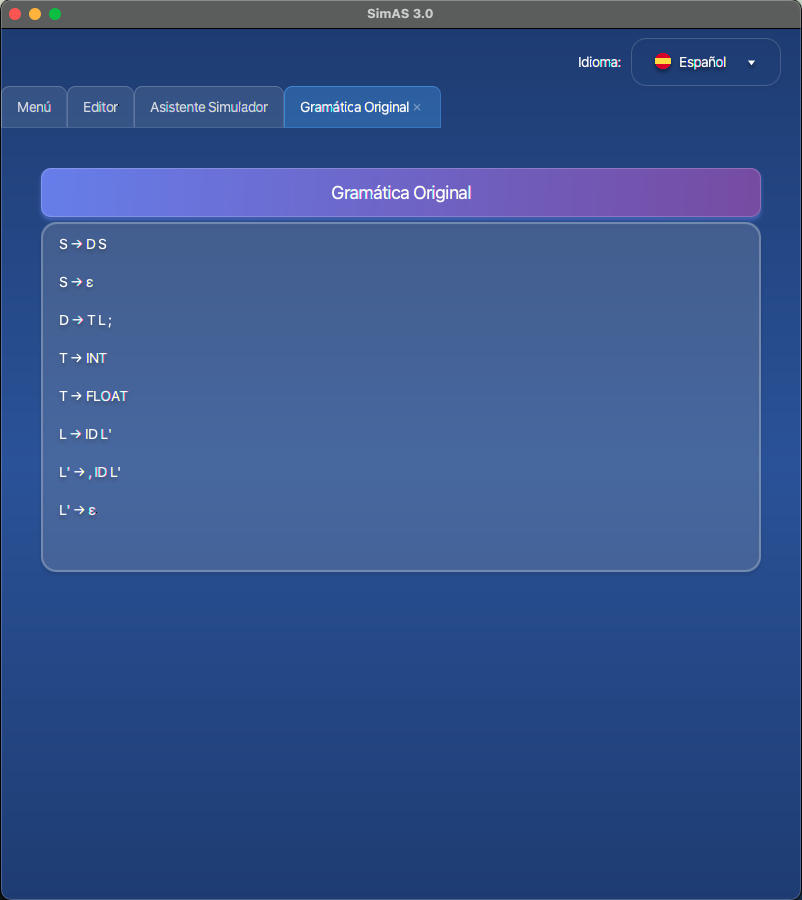
\includegraphics[width=0.9\textwidth]{figuras/simulador/gramatica_original.png}
    \caption{Vista de la gramática original desde el botón \string"Gramática\string".}
    \label{fig:gramatica_original}
\end{figure}

\subsection{Paso 1: Refactorización y eliminación de recursividad}

El primer paso del asistente constituye la fase más crítica del proceso, donde el simulador procesa la gramática original aplicando transformaciones algorítmicas avanzadas para prepararla adecuadamente para el análisis LL(1). Este paso es fundamental porque determina la viabilidad del análisis predictivo y establece las bases para todos los cálculos posteriores.

\subsubsection{Procesos realizados}

El simulador ejecuta una secuencia de algoritmos especializados:

\begin{itemize}
    \item \textbf{Eliminación de recursividad izquierda}: implementa algoritmos avanzados que detectan y eliminan tanto recursividad directa como indirecta, transformando la gramática en una forma equivalente que no presenta este problema estructural.
    \item \textbf{Factorización de producciones}: aplica técnicas de factorización para identificar y resolver producciones con prefijos comunes, eliminando ambigüedades que podrían causar conflictos en la tabla predictiva.
    \item \textbf{Validación LL(1)}: ejecuta un análisis exhaustivo para verificar que la gramática resultante cumple con todas las condiciones necesarias para ser LL(1), incluyendo la ausencia de conflictos en la tabla predictiva.
\end{itemize}

\subsubsection{Interfaz del paso 1}

La interfaz del primer paso, ilustrada en la figura \ref{fig:paso1_refactorizacion}, presenta una vista comprensiva del proceso de transformación:

\begin{itemize}
    \item \textbf{Gramática refactorizada}: muestra la gramática completamente transformada con todas las modificaciones aplicadas, permitiendo al usuario verificar la corrección de las transformaciones.
    \item \textbf{Estado de la gramática}: proporciona indicadores visuales claros sobre la validez y completitud de la gramática, incluyendo métricas de calidad y advertencias sobre posibles problemas.
    \item \textbf{Detalles de transformaciones}: presenta información detallada sobre cada cambio realizado, incluyendo el tipo de transformación aplicada y su justificación algorítmica.
\end{itemize}

\needspace{8cm}
\begin{figure}[H]
    \centering
    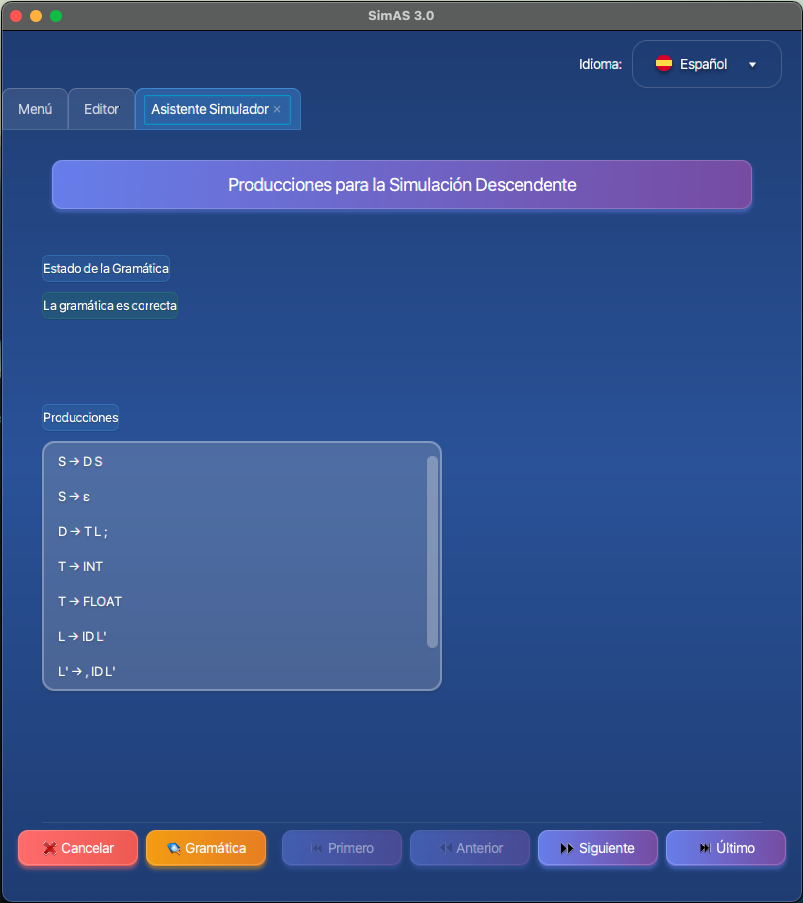
\includegraphics[width=0.9\textwidth]{figuras/simulador/paso1_recursividad_factorizacion.png}
    \caption{Paso 1: Refactorización y eliminación de recursividad}
    \label{fig:paso1_refactorizacion}
\end{figure}

\subsection{Paso 2: Construcción de conjuntos PRIMERO y SIGUIENTE}

El segundo paso representa el núcleo computacional del análisis LL(1), donde el simulador calcula los conjuntos PRIMERO y SIGUIENTE utilizando algoritmos optimizados. Estos conjuntos son fundamentales para la construcción de la tabla predictiva, ya que determinan qué producción aplicar en cada situación durante el análisis.

\subsubsection{Conjunto PRIMERO}

El conjunto PRIMERO de un símbolo $\alpha$, denotado como $PRIMERO(\alpha)$, contiene todos los símbolos terminales que pueden aparecer como primer símbolo en las derivaciones de $\alpha$. El cálculo de PRIMERO es crucial porque determina las condiciones bajo las cuales una producción puede ser aplicada durante el análisis descendente.

El algoritmo implementado maneja casos especiales como:
\begin{itemize}
    \item Símbolos terminales: $PRIMERO(a) = \{a\}$ para cualquier terminal $a$.
    \item Símbolos no terminales: cálculo recursivo considerando todas las producciones.
    \item Cadenas de símbolos: propagación de PRIMERO a través de concatenaciones.
    \item Manejo de $\varepsilon$: inclusión de $\varepsilon$ cuando es derivable.
\end{itemize}

\subsubsection{Conjunto SIGUIENTE}

El conjunto SIGUIENTE de un símbolo no terminal $A$, denotado como $SIGUIENTE(A)$, contiene todos los símbolos terminales que pueden aparecer inmediatamente después de $A$ en alguna derivación desde el símbolo inicial. SIGUIENTE es esencial para manejar producciones que derivan $\varepsilon$.

El algoritmo considera:
\begin{itemize}
    \item El símbolo inicial: $\$ \in SIGUIENTE(S)$ donde $S$ es el símbolo inicial.
    \item Propagación a través de producciones: si $A \rightarrow \alpha B \beta$, entonces $PRIMERO(\beta) \subseteq SIGUIENTE(B)$.
    \item Propagación de $\varepsilon$: si $A \rightarrow \alpha B$ y $\varepsilon \in PRIMERO(\beta)$, entonces $SIGUIENTE(A) \subseteq SIGUIENTE(B)$.
\end{itemize}

\subsubsection{Interfaz del paso 2}

La interfaz del segundo paso, mostrada en la figura \ref{fig:paso2_conjuntos}, presenta los resultados del cálculo de manera clara y organizada:

\begin{itemize}
    \item \textbf{Conjuntos PRIMERO}: presentación tabular de todos los conjuntos PRIMERO calculados para cada símbolo no terminal, con indicadores visuales para símbolos especiales como $\varepsilon$.
    \item \textbf{Conjuntos SIGUIENTE}: visualización completa de todos los conjuntos SIGUIENTE, organizados de manera que facilite la verificación manual y la comprensión de las relaciones entre símbolos.
\end{itemize}

\needspace{8cm}
\begin{figure}[H]
    \centering
    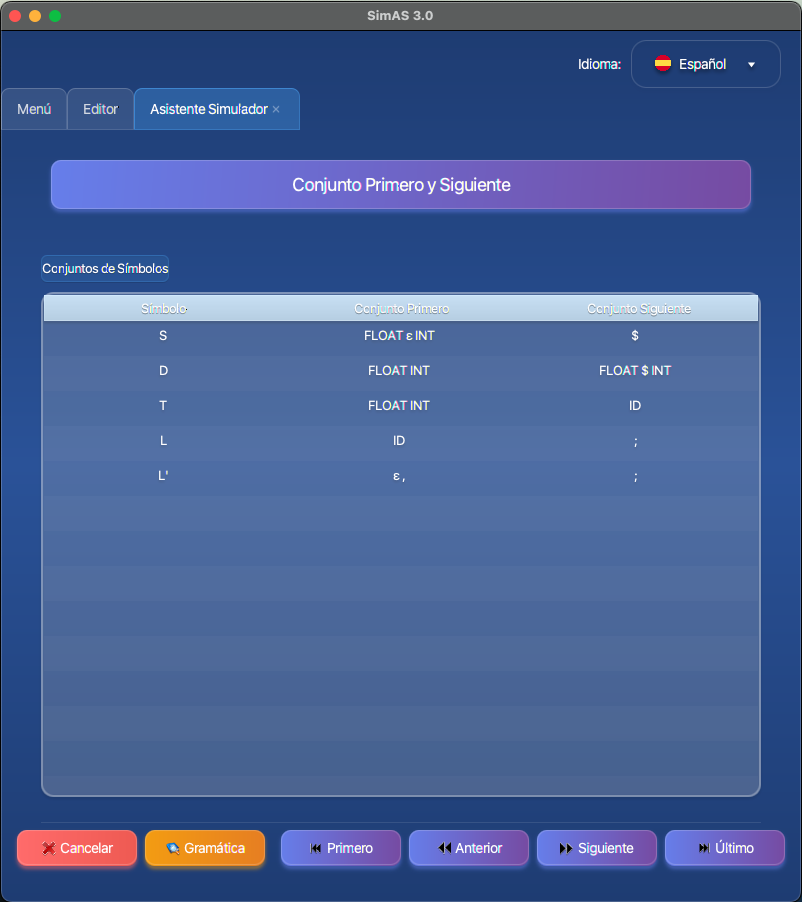
\includegraphics[width=0.9\textwidth]{figuras/simulador/paso2_conjuntos.png}
    \caption{Paso 2: Construcción de conjuntos PRIMERO y SIGUIENTE}
    \label{fig:paso2_conjuntos}
\end{figure}

\subsection{Paso 3: Construcción de la tabla predictiva}

El tercer paso representa la culminación del proceso de preparación, donde el simulador construye la tabla de análisis predictivo utilizando los conjuntos PRIMERO y SIGUIENTE calculados en el paso anterior. Esta tabla es el corazón del analizador LL(1), ya que determina de manera determinista qué acción tomar en cada situación durante el análisis.

\subsubsection{Algoritmo de construcción}

La tabla predictiva $M$ se construye aplicando un algoritmo sistemático que garantiza la corrección y completitud:

\begin{enumerate}
    \item \textbf{Inicialización}: todas las entradas de la tabla se inicializan como vacías.
    \item \textbf{Construcción para cada producción}: para cada producción $A \rightarrow \alpha$:
    \begin{itemize}
        \item Si $a \in PRIMERO(\alpha)$ y $a \neq \varepsilon$, entonces $M[A,a] = A \rightarrow \alpha$.
        \item Si $\varepsilon \in PRIMERO(\alpha)$ y $a \in SIGUIENTE(A)$, entonces $M[A,a] = A \rightarrow \alpha$.
    \end{itemize}
    \item \textbf{Detección de conflictos}: el algoritmo detecta automáticamente conflictos (múltiples producciones para la misma entrada) y los reporta al usuario.
    \item \textbf{Validación LL(1)}: verifica que la tabla resultante define una función total, confirmando que la gramática es LL(1).
\end{enumerate}

\subsubsection{Interfaz del paso 3}

La interfaz del tercer paso, ilustrada en la figura \ref{fig:paso3_tabla_predictiva}, presenta la tabla predictiva de manera intuitiva y educativa:

\begin{itemize}
    \item \textbf{Tabla predictiva completa}: matriz bidimensional que muestra la intersección de símbolos no terminales (filas) y terminales (columnas), con cada celda conteniendo la producción correspondiente o indicando que está vacía.
    \item \textbf{Producciones asignadas}: cada celda no vacía muestra claramente la producción que debe aplicarse, facilitando la comprensión del proceso de análisis y la verificación manual de la corrección.
    \item \textbf{Indicadores visuales}: uso de colores y símbolos para distinguir entre diferentes tipos de entradas y facilitar la identificación de patrones en la tabla.
\end{itemize}

\needspace{8cm}
\begin{figure}[H]
    \centering
    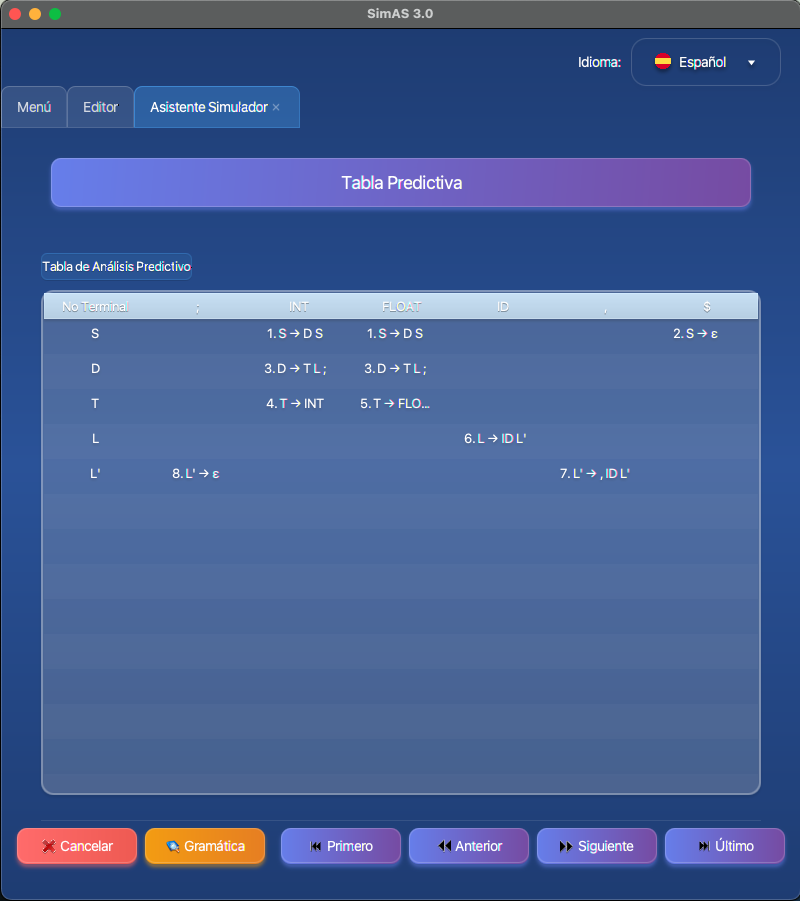
\includegraphics[width=0.9\textwidth]{figuras/simulador/paso3_tablaPredictiva.png}
    \caption{Paso 3: Construcción de la tabla predictiva}
    \label{fig:paso3_tabla_predictiva}
\end{figure}

\subsection{Paso 4: Funciones de error}

El cuarto paso introduce una funcionalidad avanzada que permite configurar un sistema sofisticado de recuperación de errores. Aunque este paso es opcional, su implementación mejora significativamente la experiencia de simulación al proporcionar mecanismos robustos para manejar cadenas de entrada que no pertenecen al lenguaje definido por la gramática.

\subsubsection{Funciones de error del sistema}

El sistema incluye un conjunto predefinido de funciones de error que implementan estrategias estándar de recuperación:

\begin{itemize}
    \item \textbf{Error de inserción}: inserta automáticamente un símbolo terminal esperado en la posición actual, permitiendo que el análisis continúe. Esta función es útil cuando falta un símbolo obligatorio.
    \item \textbf{Error de eliminación}: elimina un símbolo terminal inesperado de la entrada, saltándolo para continuar con el siguiente símbolo. Ideal para manejar símbolos extra o mal posicionados.
    \item \textbf{Error de reemplazo}: reemplaza un símbolo terminal inesperado por otro esperado, manteniendo la posición en la entrada. Útil para correcciones de símbolos similares o errores tipográficos.
\end{itemize}

\subsubsection{Panel de funciones de error}

Al hacer clic en \string"Nueva\string", se abre un panel auxiliar especializado, como se puede observar en las figuras \ref{fig:panel_funciones_error} y \ref{fig:panel_funciones_error_vacio}, que permite:

\begin{itemize}
    \item \textbf{Asignación automática de ID}: el sistema asigna automáticamente el siguiente identificador disponible, garantizando la unicidad y evitando conflictos de nomenclatura.
    \item \textbf{Definición de la función}: interfaz intuitiva para especificar el comportamiento detallado de la función de error, incluyendo condiciones de activación y acciones a realizar.
    \item \textbf{Validación en tiempo real}: verificación automática de que la función definida sea sintácticamente correcta y semánticamente válida antes de permitir su guardado.
    \item \textbf{Guardado seguro}: confirmación y almacenamiento de la función en el sistema, con verificación de integridad y compatibilidad con la gramática actual.
\end{itemize}

\needspace{8cm}
\begin{figure}[H]
    \centering
    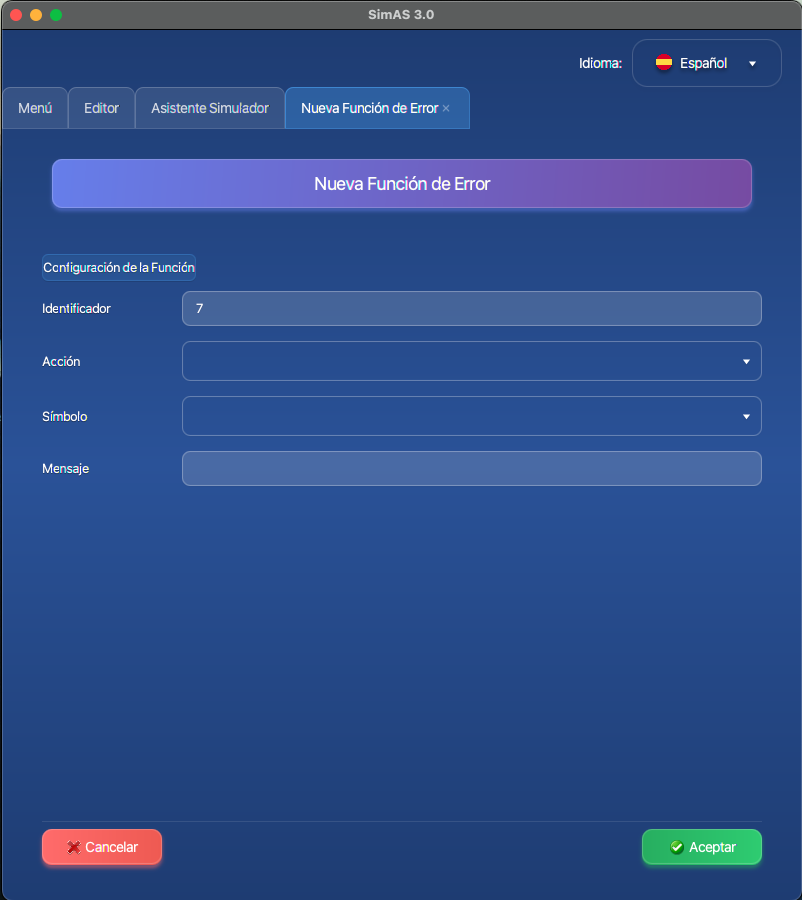
\includegraphics[width=0.9\textwidth]{figuras/simulador/panelFuncError.png}
    \caption{Panel auxiliar para crear nuevas funciones de error}
    \label{fig:panel_funciones_error}
\end{figure}

\needspace{8cm}
\begin{figure}[H]
    \centering
    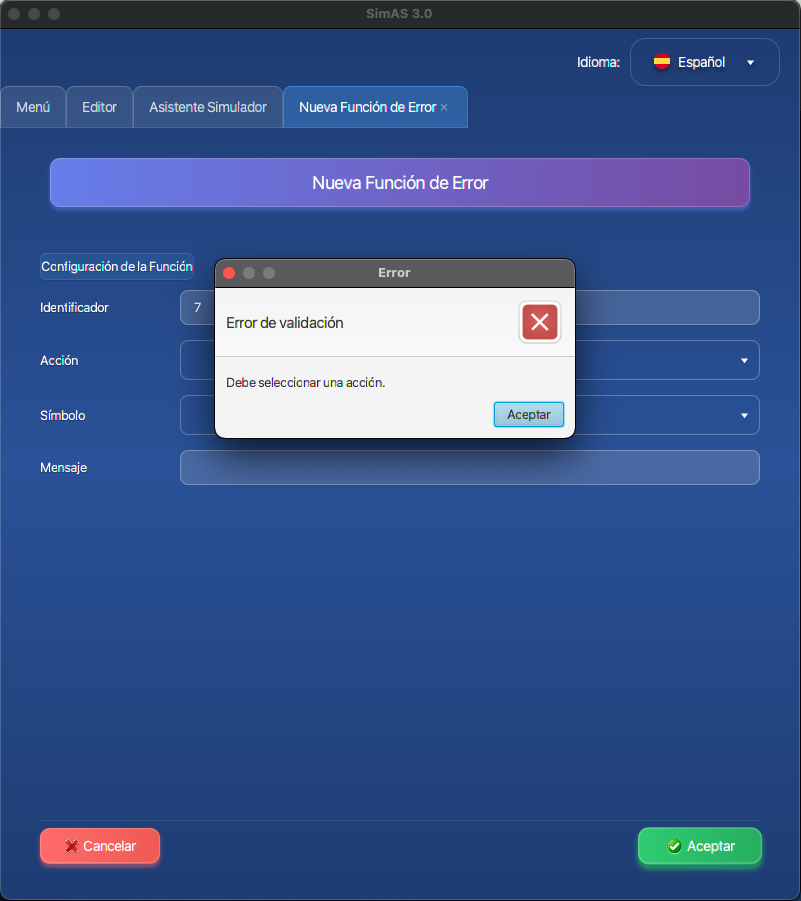
\includegraphics[width=0.9\textwidth]{figuras/simulador/panelFuncError_vacia.png}
    \caption{Panel de funciones de error en estado vacío}
    \label{fig:panel_funciones_error_vacio}
\end{figure}

\subsubsection{Gestión de funciones de error}

El sistema de gestión, ilustrado en las figuras \ref{fig:paso4_funciones_error} y \ref{fig:paso4_sin_funciones_error}, permite al usuario:

\begin{itemize}
    \item \textbf{Añadir nuevas funciones}: capacidad de crear funciones personalizadas de recuperación que se adapten a necesidades específicas o casos de uso particulares.
    \item \textbf{Eliminar funciones}: funcionalidad para quitar funciones no deseadas o que han demostrado ser problemáticas durante las pruebas.
    \item \textbf{Omitir funciones de error}: opción de continuar sin sistema de recuperación para análisis más estrictos o cuando se desea que el analizador falle inmediatamente ante errores.
\end{itemize}

\needspace{8cm}
\begin{figure}[H]
    \centering
    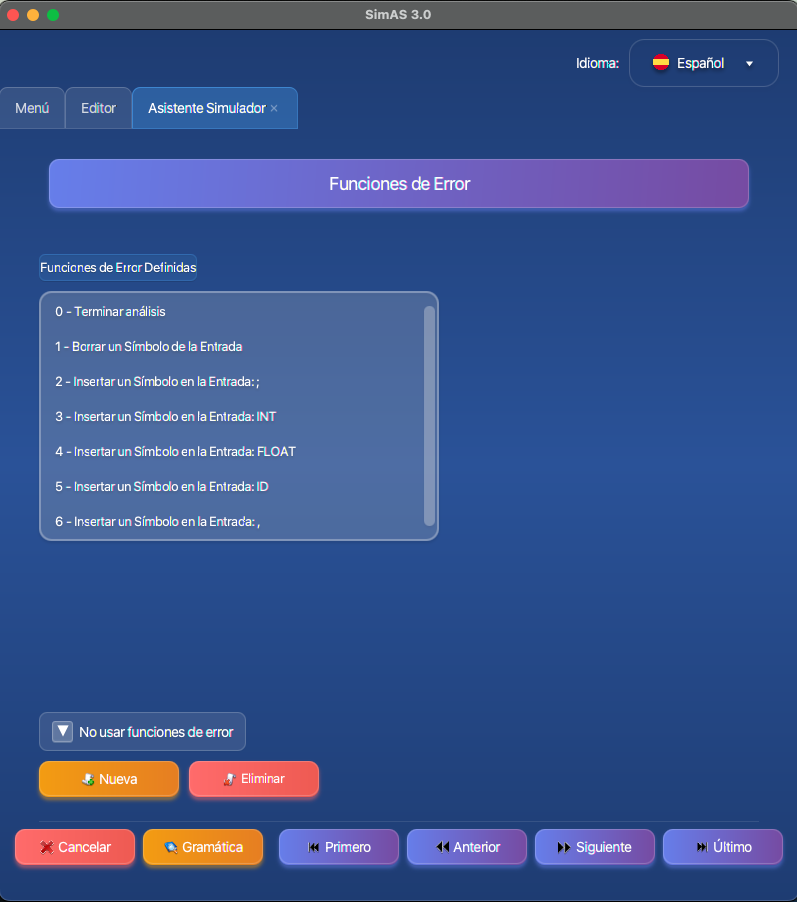
\includegraphics[width=0.9\textwidth]{figuras/simulador/paso4_funcionesError.png}
    \caption{Paso 4: Configuración de funciones de error}
    \label{fig:paso4_funciones_error}
\end{figure}

\needspace{8cm}
\begin{figure}[H]
    \centering
    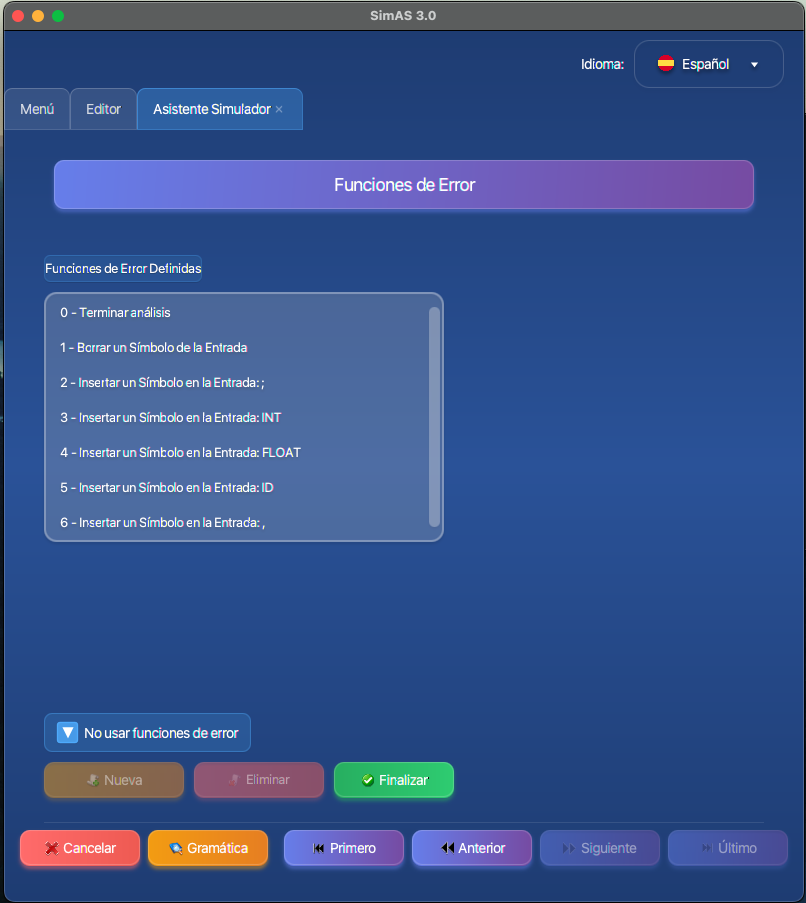
\includegraphics[width=0.9\textwidth]{figuras/simulador/paso4_no_usar_funError.png}
    \caption{Paso 4: Opción de no usar funciones de error}
    \label{fig:paso4_sin_funciones_error}
\end{figure}

\subsection{Paso 5: Tabla predictiva completa}

El quinto y último paso del asistente presenta la tabla predictiva final en su forma completa, integrando todas las producciones calculadas con las funciones de error configuradas. Este paso proporciona al usuario la oportunidad de realizar ajustes finales y personalizaciones antes de proceder con la simulación, asegurando que la configuración sea exactamente como se desea.

\subsubsection{Interfaz del paso 5}

La interfaz del paso final, mostrada en la figura \ref{fig:paso5_tabla_completa}, presenta una vista comprensiva y editable de la tabla predictiva:

\begin{itemize}
    \item \textbf{Tabla predictiva completa}: visualización integral que combina todas las producciones calculadas con las funciones de error configuradas, proporcionando una vista unificada del comportamiento del analizador.
    \item \textbf{Celdas editables interactivas}: cada celda de la tabla es clickeable, permitiendo al usuario añadir, modificar o eliminar funciones de error en posiciones específicas según sus necesidades.
    \item \textbf{Herramientas de edición avanzadas}: conjunto completo de herramientas para modificar la tabla, incluyendo operaciones de edición masiva y validación en tiempo real.
    \item \textbf{Vista previa en tiempo real}: representación visual que se actualiza instantáneamente con cada modificación, permitiendo al usuario verificar inmediatamente el impacto de sus cambios.
\end{itemize}

\needspace{8cm}
\begin{figure}[H]
    \centering
    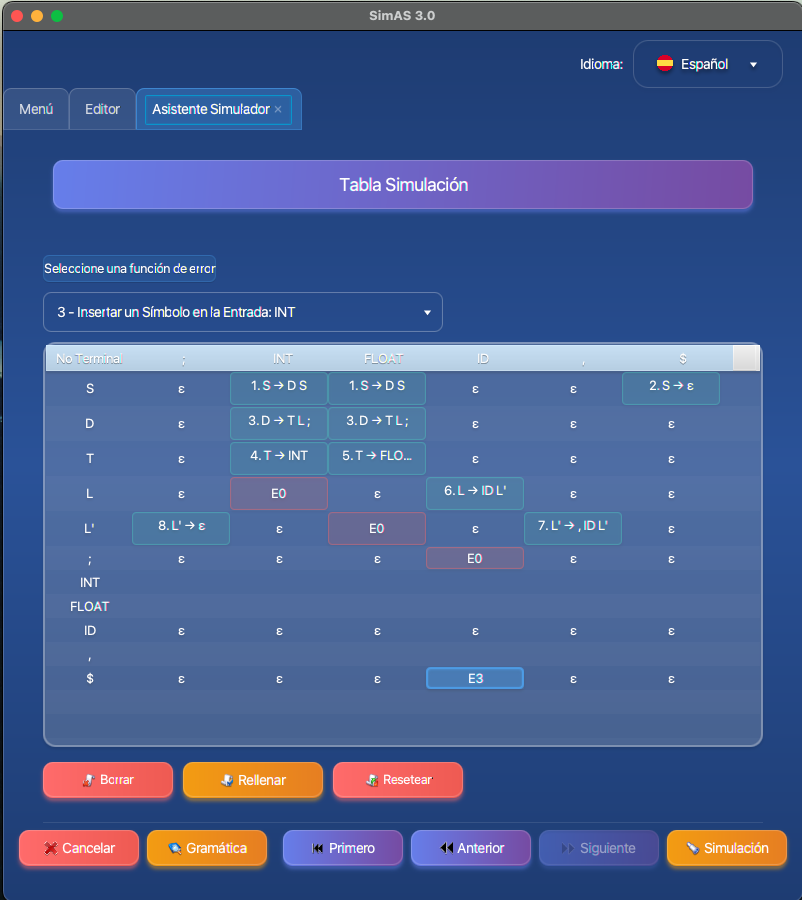
\includegraphics[width=0.9\textwidth]{figuras/simulador/paso5_tablaPredictivaCompleta.png}
    \caption{Paso 5: Tabla predictiva completa con herramientas de edición}
    \label{fig:paso5_tabla_completa}
\end{figure}

\subsubsection{Herramientas de edición}

El paso 5 incorpora un conjunto sofisticado de herramientas de edición diseñadas para facilitar la personalización de la tabla:

\begin{itemize}
    \item \textbf{Borrar selectivo}: elimina el contenido de una celda seleccionada, restringido únicamente a funciones de error para preservar la integridad de las producciones fundamentales.
    \item \textbf{Resetear a estado original}: restaura la tabla a su configuración inicial, manteniendo solo las producciones básicas y eliminando todas las funciones de error añadidas.
    \item \textbf{Rellenar con epsilon}: llena las celdas vacías con símbolos epsilon para mejorar la legibilidad visual, aunque esta operación es puramente cosmética.
\end{itemize}

\section{Simulador principal}

Una vez completados exitosamente los 5 pasos del asistente, el usuario accede al simulador principal, que representa el núcleo operativo del sistema. Esta transición se realiza mediante el botón \string"Simulación\string", que activa el entorno de simulación con toda la configuración previamente establecida.

\subsection{Interfaz del simulador}

El simulador principal, ilustrado en la figura \ref{fig:simulador_principal}, presenta una interfaz diseñada para proporcionar acceso inmediato a todas las funcionalidades esenciales:

\begin{itemize}
    \item \textbf{Resumen de configuración}: panel comprensivo que muestra las producciones modificadas, las funciones de error configuradas y la tabla predictiva final, proporcionando una vista de conjunto de toda la configuración.
    \item \textbf{Botón \string"Informe\string"}: genera automáticamente un informe PDF detallado que documenta toda la configuración y los resultados del proceso de preparación.
    \item \textbf{Botón \string"Simular\string"}: inicia el proceso de simulación interactiva, abriendo una nueva pestaña dedicada al análisis sintáctico.
\end{itemize}

\needspace{8cm}
\begin{figure}[H]
    \centering
    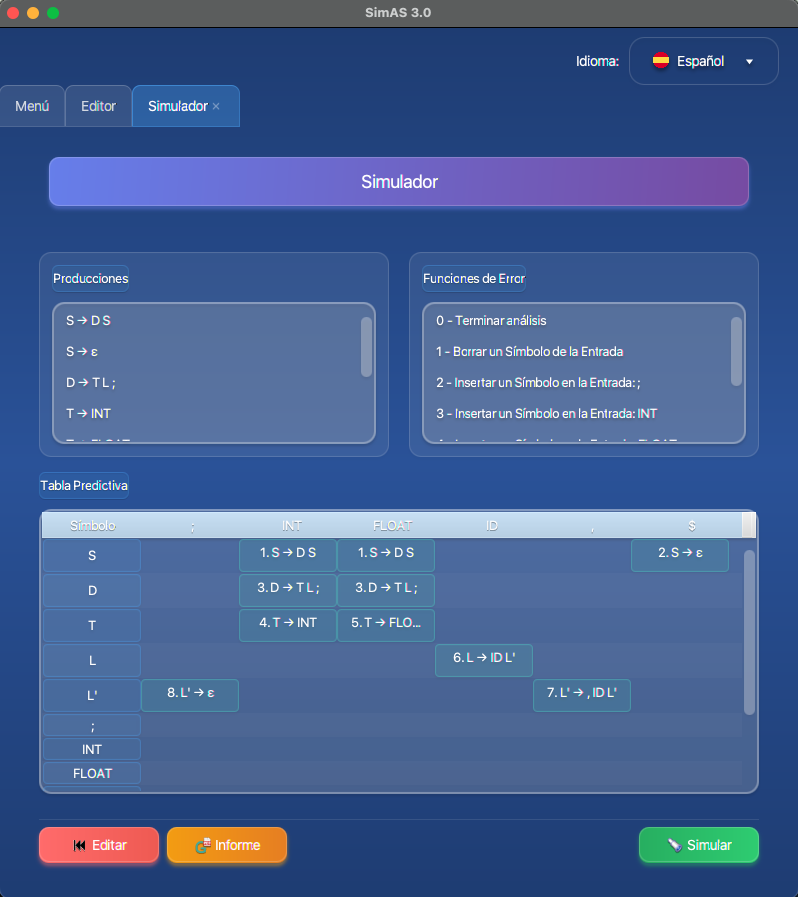
\includegraphics[width=0.9\textwidth]{figuras/simulador/simulador.png}
    \caption{Interfaz del simulador principal}
    \label{fig:simulador_principal}
\end{figure}

\subsection{Generación de informes}

El sistema de generación de informes representa una funcionalidad avanzada que produce documentación profesional y completa. El botón \string"Informe\string" genera un documento PDF estructurado que incluye:

\begin{itemize}
    \item \textbf{Información del editor}: documentación completa de la gramática original y todas las modificaciones aplicadas durante el proceso de refactorización.
    \item \textbf{Conjuntos PRIMERO y SIGUIENTE}: presentación detallada de todos los conjuntos calculados en el paso 2, con explicaciones de su significado y uso.
    \item \textbf{Tabla predictiva}: representación completa de la tabla final, incluyendo todas las producciones y funciones de error integradas.
    \item \textbf{Funciones de error}: documentación exhaustiva de todas las funciones de error configuradas, incluyendo sus definiciones, comportamientos y casos de uso.
    \item \textbf{Estadísticas y métricas}: análisis cuantitativo de la gramática y la configuración, incluyendo métricas de complejidad, cobertura y eficiencia.
\end{itemize}

\section{Simulación interactiva}

La simulación interactiva representa el corazón de la experiencia educativa de SimAS 3.0. Al hacer clic en \string"Simular\string", se abre una nueva pestaña especializada que proporciona un entorno completo para realizar análisis sintáctico con control total del usuario sobre cada aspecto del proceso.

\subsection{Interfaz de simulación}

La pestaña de simulación, mostrada en las figuras \ref{fig:simulacion_vacia} y \ref{fig:simulacion_cadena_entrada}, incorpora una interfaz intuitiva y funcional que incluye:

\begin{itemize}
    \item \textbf{Campo de entrada inteligente}: área de texto especializada para introducir la cadena a analizar, con validación en tiempo real y sugerencias de símbolos válidos.
    \item \textbf{Símbolos disponibles}: panel que muestra todos los símbolos terminales válidos para la gramática actual, facilitando la construcción de cadenas de entrada correctas.
    \item \textbf{Controles de simulación avanzados}: conjunto completo de botones para iniciar, pausar, reanudar y controlar granularmente la simulación.
    \item \textbf{Historial de pasos detallado}: registro comprensivo de cada paso del análisis, incluyendo estados intermedios y decisiones tomadas.
    \item \textbf{Navegación bidireccional}: botones para avanzar y retroceder en los pasos, permitiendo revisar y analizar cualquier momento del proceso.
\end{itemize}

\needspace{8cm}
\begin{figure}[H]
    \centering
    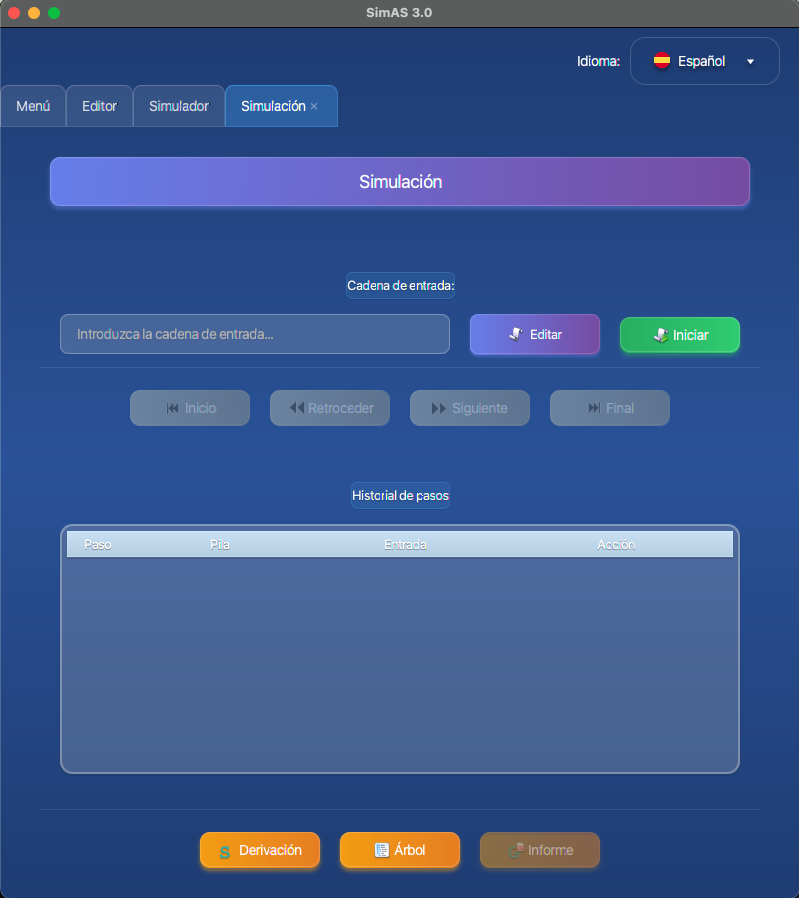
\includegraphics[width=0.9\textwidth]{figuras/simulador/simulacion_vacia.png}
    \caption{Interfaz de simulación en estado vacío}
    \label{fig:simulacion_vacia}
\end{figure}

\needspace{8cm}
\begin{figure}[H]
    \centering
    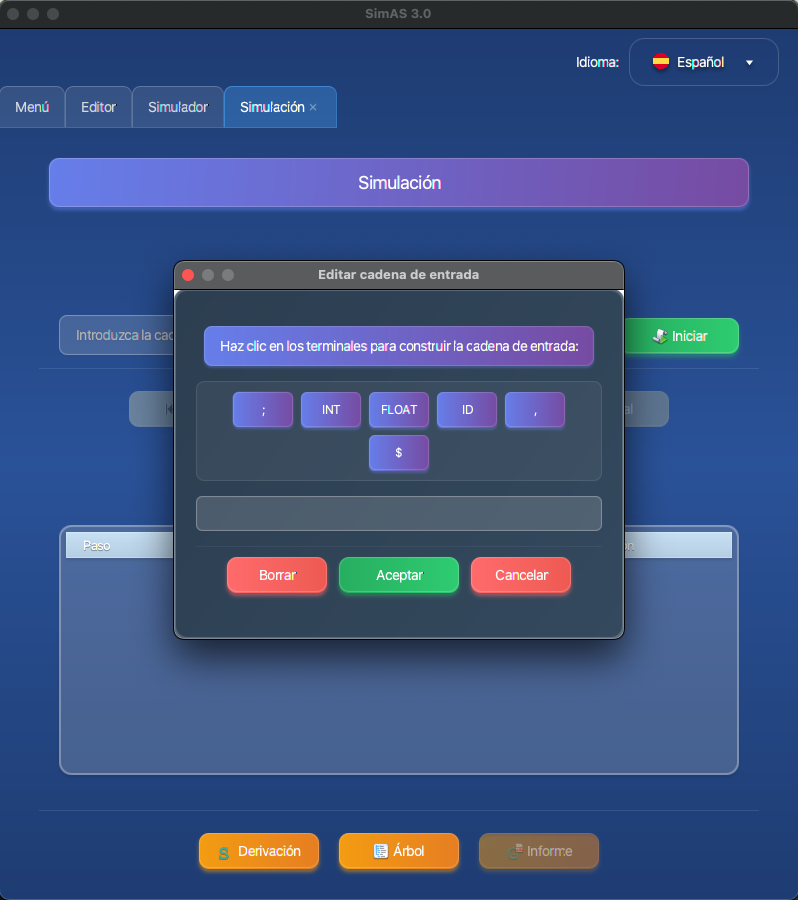
\includegraphics[width=0.9\textwidth]{figuras/simulador/simulacion_cadenaEntrada.png}
    \caption{Interfaz de simulación con cadena de entrada}
    \label{fig:simulacion_cadena_entrada}
\end{figure}

\subsection{Proceso de simulación}

El proceso de simulación implementa un algoritmo LL(1) completo que sigue una secuencia estructurada:

\begin{enumerate}
    \item \textbf{Entrada y validación de cadena}: el usuario introduce la cadena a analizar, y el sistema valida que contenga únicamente símbolos terminales válidos para la gramática.
    \item \textbf{Inicialización del analizador}: se configura la pila de análisis con el símbolo inicial y se prepara el entorno de simulación.
    \item \textbf{Ejecución del algoritmo LL(1)}: el analizador procesa la cadena utilizando la tabla predictiva, aplicando producciones y funciones de error según sea necesario.
    \item \textbf{Control interactivo}: el usuario mantiene control total sobre el avance de la simulación, pudiendo pausar, avanzar paso a paso o retroceder en cualquier momento.
    \item \textbf{Resultado final}: el sistema determina si la cadena es aceptada o rechazada, proporcionando detalles completos del proceso y estadísticas del análisis.
\end{enumerate}

\subsection{Historial de pasos}

El sistema de historial, ilustrado en la figura \ref{fig:simulacion_completa}, proporciona una vista detallada de cada paso del análisis:

\begin{itemize}
    \item \textbf{Pila de análisis}: representación visual del estado actual de la pila, mostrando los símbolos pendientes de procesar.
    \item \textbf{Acción aplicada}: documentación clara de la producción o función de error utilizada en cada paso, con justificación de la decisión.
    \item \textbf{Estado del análisis}: información comprensiva sobre el progreso actual, incluyendo posición en la entrada y estado de la pila.
    \item \textbf{Métricas de rendimiento}: estadísticas en tiempo real sobre el número de pasos, eficiencia del análisis y uso de funciones de error.
\end{itemize}

\needspace{8cm}
\begin{figure}[H]
    \centering
    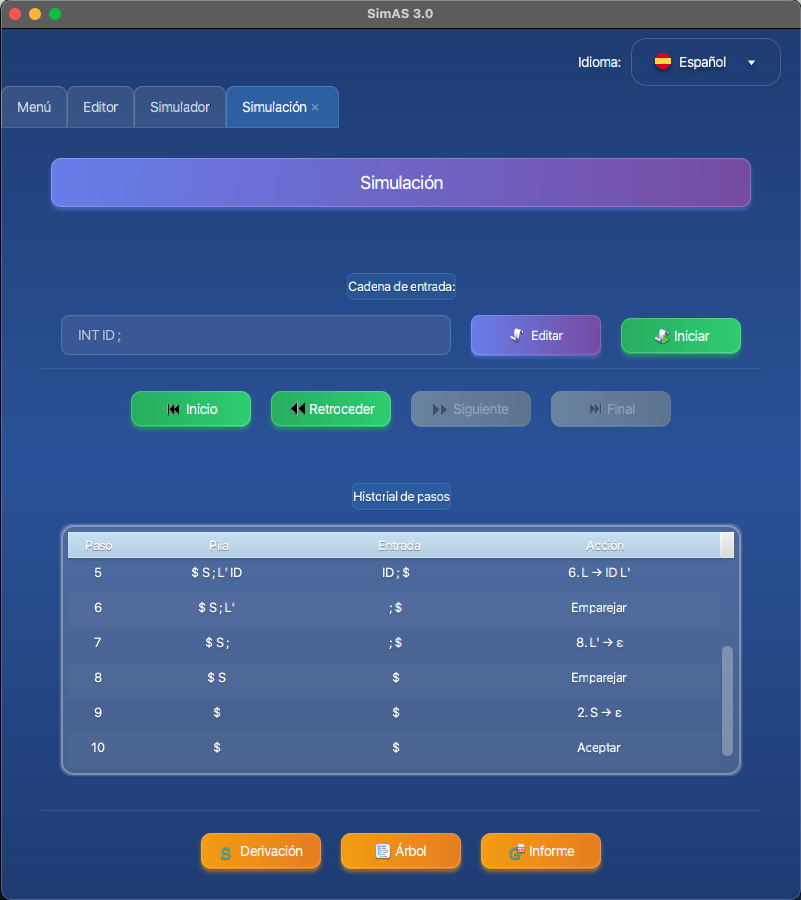
\includegraphics[width=0.9\textwidth]{figuras/simulador/simulacion_completa.png}
    \caption{Simulación completa con historial de pasos}
    \label{fig:simulacion_completa}
\end{figure}

\subsection{Navegación en la simulación}

El sistema de navegación proporciona control granular sobre la simulación:

\begin{itemize}
    \item \textbf{Avance paso a paso}: ejecuta un único paso del análisis, permitiendo al usuario examinar cada decisión en detalle.
    \item \textbf{Retroceso inteligente}: permite volver al paso anterior manteniendo la integridad del estado de la simulación.
    \item \textbf{Finalización automática}: salta al final de la simulación para obtener el resultado inmediatamente.
    \item \textbf{Reinicio completo}: restaura la simulación a su estado inicial, permitiendo comenzar de nuevo con la misma cadena o una nueva.
\end{itemize}

\section{Visualización de resultados}

El simulador incorpora un sistema avanzado de visualización que proporciona dos tipos complementarios de representación que se actualizan dinámicamente durante la simulación, facilitando la comprensión del proceso de análisis sintáctico.

\subsection{Derivación}

La derivación muestra la secuencia de producciones aplicadas durante el análisis, como se puede observar en la figura \ref{fig:simulacion_derivacion}:

\begin{itemize}
    \item \textbf{Acceso directo}: botón \string"Derivación\string" en la pestaña de simulación que abre una nueva pestaña dedicada.
    \item \textbf{Actualización automática}: se actualiza en tiempo real conforme avanza la simulación, mostrando cada paso de derivación.
    \item \textbf{Formato BNF estándar}: representación clara y estándar de cada paso de derivación, facilitando la comprensión del proceso.
    \item \textbf{Navegación sincronizada}: los cambios en la derivación reflejan exactamente la posición actual en la simulación, manteniendo la coherencia.
\end{itemize}

\needspace{8cm}
\begin{figure}[H]
    \centering
    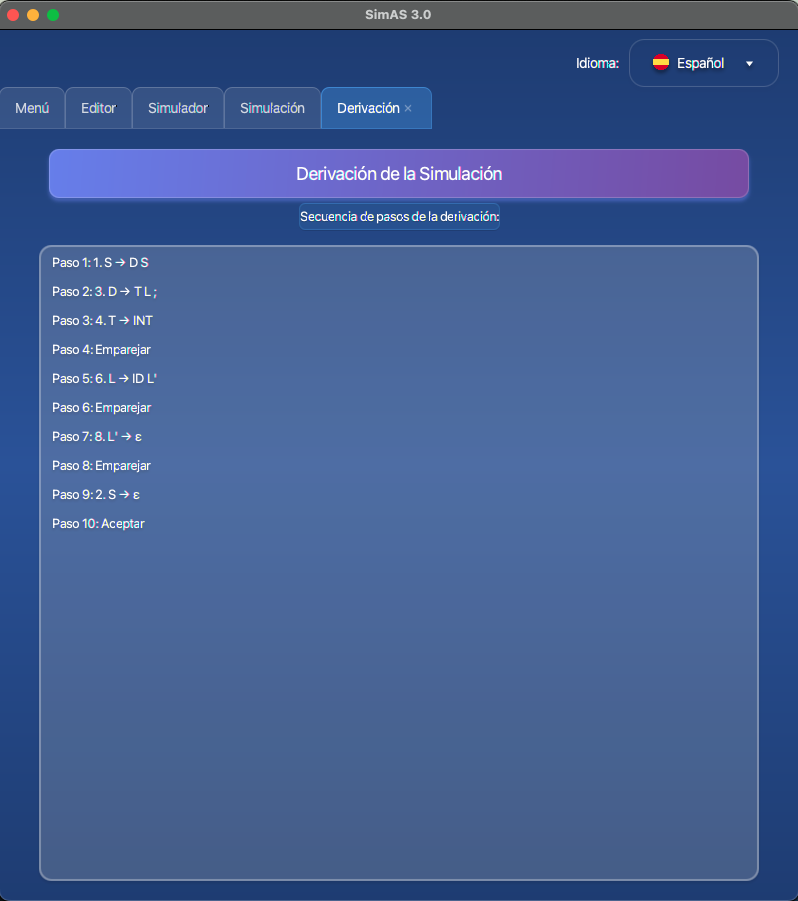
\includegraphics[width=0.9\textwidth]{figuras/simulador/simulacion_derivacion.png}
    \caption{Vista de la derivación durante la simulación}
    \label{fig:simulacion_derivacion}
\end{figure}

\subsection{Árbol sintáctico}

El árbol sintáctico proporciona una representación visual de la estructura de la cadena, ilustrado en la figura \ref{fig:simulacion_arbol}:

\begin{itemize}
    \item \textbf{Acceso directo}: botón \string"Árbol\string" en la pestaña de simulación que abre una nueva pestaña dedicada.
    \item \textbf{Construcción progresiva}: se construye paso a paso durante la simulación, mostrando el crecimiento del árbol en tiempo real.
    \item \textbf{Representación gráfica avanzada}: estructura jerárquica clara y legible con elementos visuales que facilitan la comprensión.
    \item \textbf{Sincronización perfecta}: refleja exactamente el estado actual de la simulación, manteniendo la coherencia con la derivación.
\end{itemize}

\needspace{8cm}
\begin{figure}[H]
    \centering
    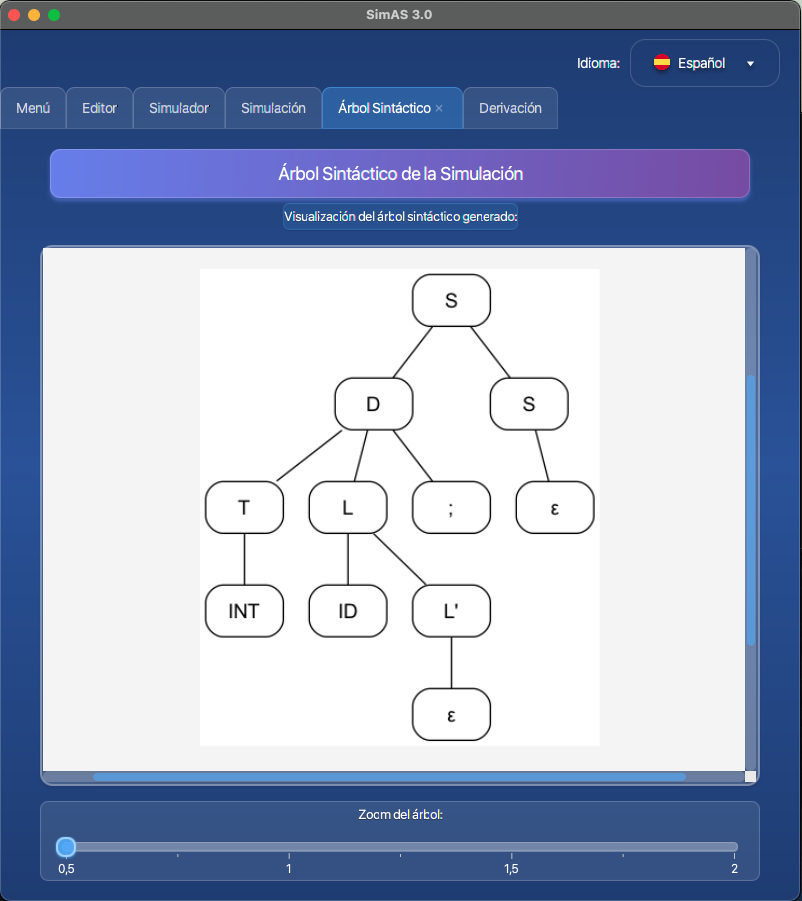
\includegraphics[width=0.9\textwidth]{figuras/simulador/simulacion_arbol.png}
    \caption{Vista del árbol sintáctico durante la simulación}
    \label{fig:simulacion_arbol}
\end{figure}

\section{Múltiples simulaciones}

Una característica avanzada y distintiva del simulador es la capacidad de manejar múltiples simulaciones simultáneamente, proporcionando una experiencia de análisis comparativo y exhaustivo que no se encuentra en herramientas similares.

\subsection{Gestión de simulaciones}

Para cada configuración de simulador, el sistema permite una gestión sofisticada:

\begin{itemize}
    \item \textbf{Crear nuevas simulaciones}: capacidad de simular diferentes cadenas de entrada manteniendo la misma configuración de gramática y funciones de error.
    \item \textbf{Mantener simulaciones activas}: múltiples simulaciones pueden estar abiertas simultáneamente, cada una en su propia pestaña independiente.
    \item \textbf{Comparar resultados}: análisis comparativo de diferentes cadenas con la misma gramática, facilitando la identificación de patrones y comportamientos.
    \item \textbf{Gestión independiente}: cada simulación mantiene su propio estado, historial y visualizaciones, permitiendo análisis paralelos sin interferencias.
\end{itemize}

\subsection{Ventajas de múltiples simulaciones}

Esta funcionalidad avanzada, mostrada en la figura \ref{fig:simulacion_varias}, permite:

\begin{itemize}
    \item \textbf{Análisis comparativo avanzado}: probar diferentes cadenas con la misma gramática, facilitando la identificación de patrones y comportamientos específicos.
    \item \textbf{Validación exhaustiva}: verificar el comportamiento del analizador con múltiples casos de prueba, incluyendo casos límite y escenarios complejos.
    \item \textbf{Experimentos educativos}: explorar diferentes escenarios de análisis, permitiendo a los estudiantes comprender mejor los conceptos teóricos.
    \item \textbf{Eficiencia operativa}: no es necesario reconfigurar el simulador para cada nueva cadena, optimizando el flujo de trabajo y la productividad.
\end{itemize}

\needspace{8cm}
\begin{figure}[H]
    \centering
    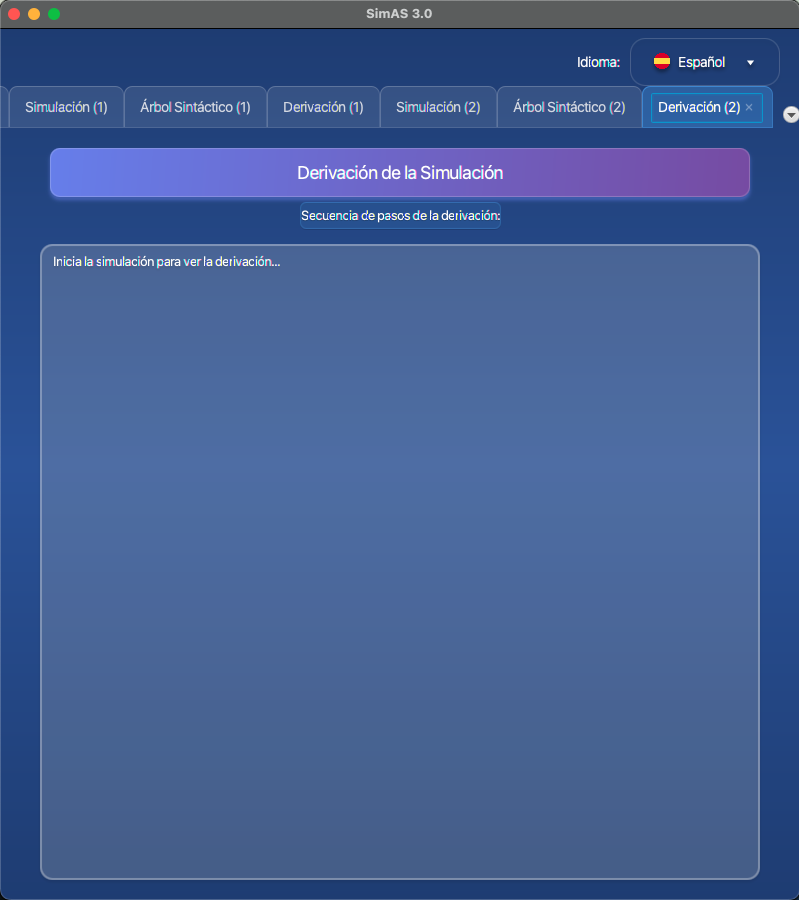
\includegraphics[width=0.9\textwidth]{figuras/simulador/simulacion_varias.png}
    \caption{Ejemplo de múltiples simulaciones simultáneas}
    \label{fig:simulacion_varias}
\end{figure}

\section{Integración con el editor}

El simulador mantiene una integración profunda y transparente con el editor de gramáticas, creando un flujo de trabajo unificado y eficiente:

\begin{itemize}
    \item \textbf{Transición automática}: paso directo y sin interrupciones del editor al simulador, manteniendo toda la configuración y estado.
    \item \textbf{Sincronización de datos en tiempo real}: cambios realizados en el editor se reflejan inmediatamente en el simulador, garantizando la coherencia.
    \item \textbf{Consistencia garantizada}: el sistema asegura que la gramática simulada es exactamente la misma que la editada, eliminando errores de configuración.
    \item \textbf{Flujo de trabajo optimizado}: proceso continuo y fluido desde la creación y edición de gramáticas hasta su simulación y análisis.
\end{itemize}

\section{Resolución de problemas}

El simulador incluye un sistema robusto de detección y resolución de problemas que ayuda a los usuarios a identificar y solucionar dificultades comunes durante el proceso de simulación.

\subsection{Problemas comunes}

El sistema está diseñado para manejar y resolver automáticamente los siguientes problemas típicos:

\begin{itemize}
    \item \textbf{Gramática no LL(1)}: el sistema detecta automáticamente conflictos en la tabla predictiva y proporciona sugerencias específicas para resolverlos.
    \item \textbf{Recursividad no eliminable}: se informa al usuario sobre limitaciones estructurales y se sugieren alternativas de diseño.
    \item \textbf{Funciones de error incorrectas}: validación automática previene errores de configuración y proporciona retroalimentación detallada.
    \item \textbf{Cadenas inválidas}: el sistema valida la entrada antes de la simulación y proporciona información específica sobre símbolos no válidos.
\end{itemize}

\subsection{Soluciones recomendadas}

Para resolver problemas comunes, se recomiendan las siguientes estrategias:

\begin{itemize}
    \item \textbf{Revisar la gramática}: verificar que la gramática sea LL(1) utilizando las herramientas de validación del editor.
    \item \textbf{Ajustar funciones de error}: modificar o eliminar funciones problemáticas utilizando el panel de gestión del paso 4.
    \item \textbf{Validar entrada}: asegurar que la cadena contenga únicamente símbolos terminales válidos para la gramática actual.
    \item \textbf{Consultar la documentación}: revisar ejemplos y casos de uso para comprender mejor el comportamiento esperado.
\end{itemize}

\section{Conclusión}

El simulador de análisis sintáctico descendente predictivo de SimAS 3.0 representa una herramienta educativa de vanguardia que combina la potencia algorítmica del análisis LL(1) con una interfaz intuitiva y educativa de última generación. El asistente guiado de 5 pasos simplifica significativamente la configuración compleja requerida para el análisis sintáctico, mientras que las funciones avanzadas de visualización y múltiples simulaciones proporcionan una experiencia de aprendizaje rica, completa y profundamente educativa.

La integración perfecta y transparente con el editor de gramáticas, el sistema avanzado de recuperación de errores, y la capacidad de generar informes detallados y profesionales hacen del simulador una herramienta indispensable para el estudio, la práctica y la investigación del análisis sintáctico. La funcionalidad innovadora de múltiples simulaciones permite una exploración exhaustiva y comparativa de las capacidades de la gramática, mientras que la navegación paso a paso y las visualizaciones dinámicas facilitan la comprensión profunda de los conceptos teóricos subyacentes.

El simulador no solo demuestra la corrección y eficiencia de las gramáticas, sino que también educa de manera integral sobre el proceso completo de análisis sintáctico, proporcionando una base sólida y comprensiva para el aprendizaje de conceptos avanzados en teoría de lenguajes formales, compiladores y análisis sintáctico. Su diseño educativo y su implementación técnica robusta lo convierten en una herramienta de referencia para la enseñanza y el aprendizaje de estos conceptos fundamentales en ciencias de la computación.


\input{capitulos/06_Ejemplos_Prácticos}


\cleardoublepage
\addcontentsline{toc}{chapter}{Bibliografía}


%\bibliographystyle{vancouver}
%\printbibheading[heading=bibintoc]
\printbibliography

\renewcommand{\appendixpagename}{Anexos}
\renewcommand{\appendixtocname}{Anexos}
\renewcommand{\appendixname}{Anexo}

\end{document}